\documentclass[aspectratio=169,11pt]{beamer}

% Shared style (ib-tutorials.sty at the repo root).
\makeatletter\def\input@path{{./}{../}}\makeatother
\usepackage{ib-tutorials}

\usepackage[utf8]{inputenc}
\usepackage{amsmath,amssymb}
\usepackage{booktabs}
\usepackage{array}
\newcolumntype{L}[1]{>{\raggedright\arraybackslash}p{#1}}
\usepackage{graphicx}
\graphicspath{{../pictures/2-ib2d/}{pictures/2-ib2d/}}
\usepackage{xcolor}
\usepackage{listings}
\usepackage{tikz}
\usetikzlibrary{arrows.meta,positioning,shapes.geometric,fit,calc}
\usepackage{hyperref}

\newcommand{\sourcecredit}[1]{\vfill\hfill{\tiny\textcolor{DarkGray}{#1}}}

\lstset{
  basicstyle=\ttfamily\scriptsize\color{BlackGray},
  keywordstyle=\color{NavyBlue}\bfseries,
  commentstyle=\color{DarkGray}\itshape,
  stringstyle=\color{OliveGreen},
  showstringspaces=false,
  columns=fullflexible,
  keepspaces=true,
  breaklines=true,
  frame=single,
  framerule=0.4pt,
  rulecolor=\color{LightGray},
  backgroundcolor=\color{LightGray!30},
  xleftmargin=0.25em,
  xrightmargin=0.25em
}
\lstdefinestyle{shell}{morecomment=[l]{\#}}
\lstdefinestyle{input}{morecomment=[l]{\%}}
\lstdefinestyle{plain}{}
\lstdefinestyle{tiny}{basicstyle=\ttfamily\tiny\color{BlackGray}}

\title[IB2d: introduction and file formats]{Introduction to IB2d and its file formats}
\subtitle{What IB2d is and when to use it; getting it in MATLAB or Python; an example folder, \code{input2d} line by line, and every structure file (\code{.vertex}, \code{.spring}, \code{.beam}, \code{.target}, \code{.mass} and the rest); where the output goes}
\author[Miller]{Laura A. Miller}
\institute[UArizona]{Department of Mathematics, University of Arizona}
\date{Using IB Software \textbullet\ Part II \textbullet\ Chapter 4a}

\begin{document}

% ---------------------------------------------------------------- title
\begin{frame}[plain]
\maketutorialtitlepanel{%
\begin{tikzpicture}[scale=0.95]
  \draw[step=0.25,LightGray!70,very thin] (0,0) grid (4,4);
  \draw[DarkGray,thick] (0,0) rectangle (4,4);
  \draw[NavyBlue,very thick] (2,2) ellipse (0.8 and 1.55);
  \foreach \a in {0,15,...,345} {\fill[BlackGray] ({2+0.8*cos(\a)},{2+1.55*sin(\a)}) circle (1.3pt);}
  \node[font=\tiny,DarkGray,anchor=south west] at (0.05,0.05) {(0,0)};
  \node[font=\tiny,DarkGray,anchor=north east] at (3.95,3.95) {(Lx,Ly)};
  \node[font=\tiny,NavyBlue] at (2,0.35) {\code{.vertex} + \code{.spring}};
\end{tikzpicture}}
\end{frame}

% ---------------------------------------------------------------- goals
\begin{frame}{What you will be able to do after this chapter}
\label{fr:goals}
\begin{itemize}
  \item Say what IB2d is, what it models, what it does not, and when to reach for it instead of IBAMR (Part III) or IBFE (Part IV).
  \item Get the code and run its rubber-band example in MATLAB or in Python, and know what the run prints and writes.
  \item Read every line of \code{input2d}: the fluid, time, grid, structure, output and name blocks, and how the file is parsed.
  \item Write the structure files by hand or from a script: \code{.vertex} (required) and \code{.spring}, \code{.d\_spring}, \code{.beam}, \code{.nonInv\_beam}, \code{.target}, \code{.mass}, with the force law behind each, and know the names and columns of the rest.
  \item Know the one difference that bites first: the MATLAB files count points from 1, the Python files from 0.
  \item Find the output (\code{viz\_IB2d/}, \code{hier\_IB2d\_data/}) and read a file of it before chapter 4b opens them in VisIt.
\end{itemize}
\end{frame}

\begin{frame}{How these slides were checked}
\label{fr:checked}
\begin{punchbox}
\small Every format and every rule on these slides was checked against the readers in the IB2d code (\code{IBM\_Driver.m}, \code{IBM\_Driver.py}, \code{please\_Read\_input2d\_File}, \code{please\_Initialize\_Simulation}) and against runs of the four Python rubber-band examples (October 2026). Where a slide and an older deck disagree, the slide follows the code and says so.
\end{punchbox}
\footnotesize
\begin{itemize}
  \item The force laws are transcribed from \code{please\_Find\_Lagrangian\_Forces\_On\_Eulerian\_grid.m}, the delta function from \code{give\_Delta\_Kernel.m}, the parser's rules from \code{please\_Read\_input2d\_File} and the initializer, the output names from the driver's \code{print\_vtk\_files}.
  \item The runs: \code{Rubberband\_with\_Springs}, \code{\_with\_Beams}, \code{\_with\_Damped\_Springs} and \code{Wobbly\_Beam} from \code{pyIB2d/Examples}, in WSL (Ubuntu 24.04, Python 3.12, numba 0.68), plotting off; the MATLAB version was read, not run (no MATLAB on the laptop; the Octave attempt is on slide \ref{fr:octave}).
  \item The code read is the clone of 2024-03-06; the GitHub page and its news were checked in October 2026 and the repository has moved on since (973 commits), so a key name or an example may differ in detail from these slides. The checks are easy to repeat: the file names on slide \ref{fr:refs}.
\end{itemize}
\end{frame}

\begin{frame}{Where this chapter comes from (1/2)}
\label{fr:sources}
\small
\begin{itemize}
  \item \al{``Getting Running on IB2D and IBAMR'' (2016, 10 slides):} the quick start of the UNC course: clone, ``type \code{main2d}'', what IB2d can do, where the output goes. Its cluster part (Kure, LSF, \code{bmatlab}) is retired (Part X).
  \item \al{``A quick intro to ib2d'' (Lecture 9, 2021--24, 51 slides) and ``ib2d and moving the boundaries'' (Lecture 11):} the boundary description, the four IB steps, the input files, the file formats with their format pictures, the rubber-band generator, homework 4, and (in L9) a VisIt walk-through that belongs to chapter 4b.
  \item \al{``Introduction to IB2D'' (2024, 16 slides):} the same file-format slides, the three papers and the four video tutorials.
\end{itemize}
\end{frame}

\begin{frame}{Where this chapter comes from (2/2)}
\label{fr:sources2}
\small
\begin{itemize}
  \item \al{``IB2d and IBAMR associated files'' (Lecture 2, 2022, 38 slides):} the IB2d/IBAMR comparison (one list vs many files, index base, the domain's origin, $\Delta s = \Delta x/2$), the generator in both flavours, the MATLAB checkers, the project goals.
  \item \al{``ib2d part 2'' (Lecture 10, 2023):} MATLAB vs Python, the Anaconda route.
  \item \al{The IB2d repository} (\url{https://github.com/nickabattista/IB2d}; the code read here is the 2024-03-06 clone, the page checked October 2026): the README, \code{IB2d\_New\_Functionality.txt}, the example folders, and the readers in \code{IBM\_Blackbox}.
\end{itemize}
What is new here: the Python/MATLAB index difference, the input parser's rules (unknown keys, duplicates, defaults), the force laws as coded, the output file formats, timings on a laptop, and the beams-example trap (slide \ref{fr:trap}).
\end{frame}

% ---------------------------------------------------------------- what IB2d is
\begin{frame}{What IB2d is}
\label{fr:what}
\begin{columns}[T]
\column{0.58\textwidth}
\footnotesize
\begin{itemize}
  \item A two-dimensional immersed boundary code with \al{complete implementations in MATLAB and in Python}, written by Nick Battista (The College of New Jersey; started at UNC in May 2015), with the Python port by Christopher Strickland (2016).
  \item One Cartesian grid, periodic in both directions, solved with FFTs; one list of Lagrangian points carrying springs, beams, target points, masses, muscles and more (slide \ref{fr:models}).
  \item Everything is a text file: \code{input2d} and a family of \code{<name>.vertex}, \code{.spring}, \ldots; the output is VTK text that VisIt and ParaView read.
  \item ``Over 75 built-in examples'' (the README): rubber bands, channels, heart tubes, jellyfish, insects, corals, cells, a Turek--Hron flag.
  \item Licence GPL-3.0; 973 commits and 206 stars on GitHub in October 2026.
\end{itemize}
\column{0.40\textwidth}
\scriptsize
\al{Where it sits} (chapter 1b's table):

\vspace{1mm}
\begin{tabular}{@{}L{0.26\textwidth}L{0.62\textwidth}@{}}
\toprule
IB2d & 2D, MATLAB/Python, a laptop, Re up to about $10^3$; learning, elastic and muscle-driven boundaries, porous media \\
IBAMR & 2D/3D, C++ on a cluster, adaptive grids, the same fibre models and more (Part III) \\
IBFE & finite-element solids in IBAMR, 3D organs (Part IV) \\
\bottomrule
\end{tabular}

\vspace{2mm}
The 2024 deck: ``useful for 2D simulations of flexible, moving boundaries at Re $<$ 1000.''
\end{columns}
\end{frame}

\begin{frame}{The papers and the videos}
\label{fr:papers}
\footnotesize
Cite these when you use IB2d (the README asks for all three, and to let Nick Battista know):
\begin{enumerate}
  \item N. A. Battista, A. J. Baird, L. A. Miller. A mathematical model and MATLAB code for muscle-fluid-structure simulations. \emph{Integr.\ Comp.\ Biol.} 55(5):901--911, 2015 (the muscle models, slide \ref{fr:models}; chapter 4e).
  \item N. A. Battista, W. C. Strickland, L. A. Miller. IB2d: a Python and MATLAB implementation of the immersed boundary method. \emph{Bioinspir.\ Biomim.} 12(3):036003, 2017; preprint arXiv:1610.07944.
  \item N. A. Battista, W. C. Strickland, A. Barrett, L. A. Miller. IB2d Reloaded: a more powerful Python and MATLAB implementation of the immersed boundary method. \emph{Math.\ Meth.\ Appl.\ Sci.} 41(18):8455--8480, 2018; preprint arXiv:1707.06928.
\end{enumerate}
Later additions: D. M. Senter et al., MeshmerizeMe, \emph{Bioinspir.\ Biomim.} 16:016008, 2021 (chapter 4f); M. Santiago, N. A. Battista, L. A. Miller, S. Khatri, passive concentration dynamics in IB2d, \emph{Bioinspir.\ Biomim.} 17:036003, 2022.

\vspace{1mm}
\al{Nick Battista's four video tutorials} (YouTube): 1 the IB method, fibre models and IB2d (\url{https://youtu.be/PJyQA0vwbgU}); 2 what comes with IB2d, the example folders and the input files (\url{https://youtu.be/jSwCKq0v84s}); 3 building a geometry and its \code{.vertex}/\code{.spring} files from the rubber band (\url{https://youtu.be/I3TLpyEBXfE}); 4 VisIt: the points, colour maps and vectors (\url{https://youtu.be/4D4ruXbeCiQ}). Tutorials 2 and 3 cover this chapter; 4 is chapter 4b.
\sourcecredit{The older decks cite paper 3 as ``in press''; it appeared in 2018. ``Biomemetics'' in the decks is ``Biomimetics''.}
\end{frame}

\begin{frame}{How IB2d grew (from \code{IB2d\_New\_Functionality.txt} and the README news)}
\label{fr:timeline}
\begin{center}
\resizebox{0.96\textwidth}{!}{%
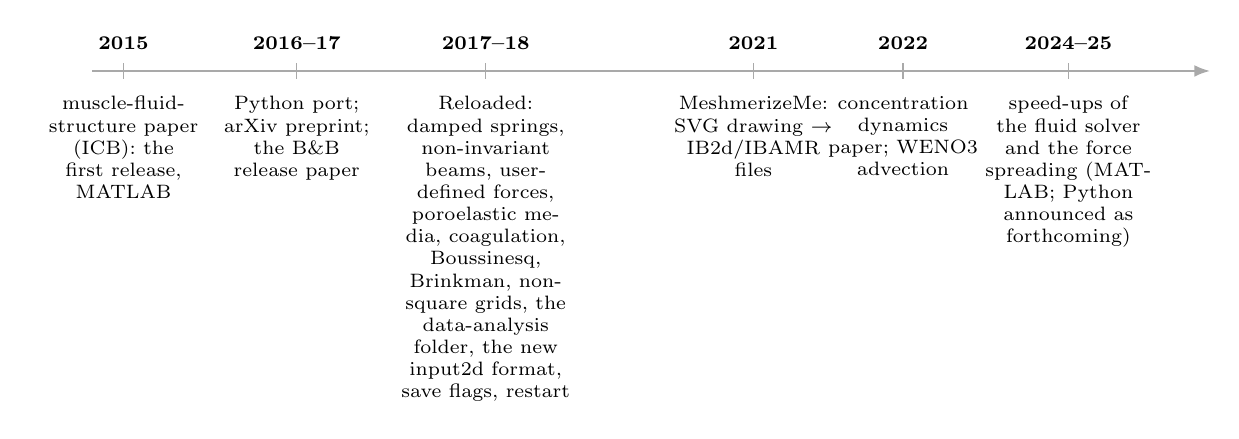
\begin{tikzpicture}[x=1cm,y=1cm,font=\scriptsize]
  \draw[DarkGray,thick,-{Latex[length=2mm]}] (0,0) -- (14.2,0);
  \foreach \x/\y/\t in {0.4/2015/{muscle-fluid-structure paper (ICB): the first release, MATLAB},
                        2.6/2016--17/{Python port; arXiv preprint; the B\&B release paper},
                        5.0/2017--18/{Reloaded: damped springs, non-invariant beams, user-defined forces, poroelastic media, coagulation, Boussinesq, Brinkman, non-square grids, the data-analysis folder, the new input2d format, save flags, restart},
                        8.4/2021/{MeshmerizeMe: SVG drawing $\to$ IB2d/IBAMR files},
                        10.3/2022/{concentration dynamics paper; WENO3 advection},
                        12.4/2024--25/{speed-ups of the fluid solver and the force spreading (MATLAB; Python announced as forthcoming)}} {
    \draw[DarkGray] (\x,0.1) -- (\x,-0.1);
    \node[anchor=south,font=\scriptsize\bfseries] at (\x,0.15) {\y};
    \node[anchor=north,text width=2.2cm,align=center] at (\x,-0.2) {\t};
  }
\end{tikzpicture}}
\end{center}
\footnotesize
\begin{itemize}
  \item The input file format changed with Reloaded (the braced blocks of slide \ref{fr:input1}); the old one-value-per-line format is still accepted (slide \ref{fr:parser}).
  \item The MATLAB code has had every feature first; the Python port follows (slide \ref{fr:mat-vs-py}).
\end{itemize}
\end{frame}

% ---------------------------------------------------------------- the idea
\begin{frame}{Describing the boundary}
\label{fr:boundary}
\begin{columns}[T]
\column{0.55\textwidth}
\footnotesize
From the 2024 deck, unchanged because it is the whole idea:
\begin{itemize}
  \item In the immersed boundary method, \al{boundaries are always elastic}.
  \item They can be stiff enough that they act like rigid objects.
  \item They can be moved in prescribed ways using \al{target points}.
  \item Boundaries have been modelled to resist bending, stretching and twisting.
  \item All of these properties can change in time, in prescribed ways or according to other models.
\end{itemize}
In IB2d every one of these is a line in a text file: a spring between two points, a beam over three, a target point tethering one point to a position, a mass attached to one point. The point list itself is the \code{.vertex} file.
\column{0.43\textwidth}
\begin{tikzpicture}[scale=0.9,font=\scriptsize]
  \draw[step=0.4,LightGray!70,very thin] (0,0) grid (4.4,3.6);
  \node[DarkGray] at (2.2,3.3) {Eulerian grid: $u(\mathbf{x},t)$, $p$, $\mathbf{f}$};
  \draw[NavyBlue,very thick] (0.6,1.2) .. controls (1.4,2.6) and (2.6,0.4) .. (3.8,1.8);
  \foreach \p in {(0.6,1.2),(0.95,1.55),(1.3,1.72),(1.65,1.68),(2.0,1.5),(2.35,1.3),(2.7,1.2),(3.05,1.28),(3.4,1.5),(3.8,1.8)} {\fill[BlackGray] \p circle (1.4pt);}
  \node[NavyBlue,anchor=north] at (2.2,0.5) {Lagrangian points: $\mathbf{X}_i(t)$, $\mathbf{F}_i$};
  \draw[-{Latex[length=1.5mm]},OliveGreen,thick] (1.3,1.72) -- (1.3,2.5) node[right,OliveGreen] {$\mathbf{F}_i$ spread to the grid};
  \draw[-{Latex[length=1.5mm]},RubineRed,thick] (3.05,1.28) -- (3.6,0.9) node[below,RubineRed] {$\mathbf{U}_i$ interpolated};
\end{tikzpicture}
\end{columns}
\end{frame}

\begin{frame}{The four steps of every time step (and what IB2d does for each)}
\label{fr:steps}
\footnotesize
\begin{enumerate}
  \item \al{Forces on the boundary} from its deformation: springs, beams, target points, \ldots (the laws on slides \ref{fr:spring}--\ref{fr:mass}); \code{please\_Find\_Lagrangian\_Forces\_On\_Eulerian\_grid}.
  \item \al{Spread} the forces to the grid with the discrete delta function (slide \ref{fr:delta}): $\mathbf{f}(\mathbf{x}) = \sum_i \mathbf{F}_i\, \delta_h(\mathbf{x} - \mathbf{X}_i)\, \Delta s$.
  \item \al{Solve the fluid}: incompressible Navier--Stokes on the periodic grid by FFT, with Peskin's two-step (half-step) scheme and the advection term in skew-symmetric form; the viscous term is treated implicitly in Fourier space; \code{please\_Update\_Fluid\_Velocity}.
  \item \al{Move the boundary} at the local fluid velocity: $\mathbf{U}_i = \sum_{\mathbf{x}} \mathbf{u}(\mathbf{x})\, \delta_h(\mathbf{x} - \mathbf{X}_i)\, \Delta x \Delta y$, then $\mathbf{X}_i \leftarrow \mathbf{X}_i + \Delta t\, \mathbf{U}_i$; \code{please\_Move\_Lagrangian\_Point\_Positions}.
\end{enumerate}
\begin{itemize}
  \item Chapter 5 and the theory repository give the equations and the accuracy; chapter 4d does the stability lab (what happens when $\Delta t$ or the stiffness is too large).
  \item IB2d's driver (\code{IBM\_Driver}) moves the points a half step with the old velocity, computes the forces once at those positions, solves the fluid once, and moves the points the full step with the new velocity: Peskin's 2002 scheme. The updates of springs, targets and beams (chapter 4c) happen at the start of each step.
  \item The structure is one list: \code{xLag}, \code{yLag} arrays in the order of the \code{.vertex} file. Every other file refers to that order.
\end{itemize}
\end{frame}

\begin{frame}{What IB2d can model (the flags in \code{input2d})}
\label{fr:models}
\scriptsize
\begin{tabular}{@{}L{0.24\textwidth}L{0.42\textwidth}L{0.26\textwidth}@{}}
\toprule
Fibre model & What it is & File, flag \\
\midrule
springs (Hookean or power-law) & two points, stiffness, resting length, optional exponent & \code{.spring}, \code{springs} \\
damped springs & the same plus a damping coefficient & \code{.d\_spring}, \code{damped\_springs} \\
beams (torsional springs) & three points, bending stiffness, a scalar rest curvature & \code{.beam}, \code{beams} \\
non-invariant beams & three points, stiffness, a rest curvature vector $(C_x, C_y)$ & \code{.nonInv\_beam}, \code{nonInvariant\_beams} \\
target points & a point tethered to a position (prescribed motion in 4c) & \code{.target}, \code{target\_pts} \\
mass points, gravity & a massive copy tethered to the point; a gravity vector & \code{.mass}, \code{mass\_pts}, \code{gravity} \\
muscles & force-velocity + length-tension (Hill); the 3-element Hill model & \code{.muscle}, \code{FV\_LT\_muscle}; \code{.3\_muscle}, \code{3\_element\_muscle} \\
porous, poroelastic & a slip velocity through the boundary; a Brinkman-like solid & \code{.porous}, \code{porous\_media}; \code{.poroelastic}, \code{poroelastic} \\
user-defined force & any force law you code & \code{.user\_force}, \code{user\_force\_model} \\
coagulation & cells that aggregate when close & \code{.coagulation}, \code{coagulation} \\
electrophysiology & FitzHugh--Nagumo activation driving muscles & \code{electro\_phys} \\
\bottomrule
\end{tabular}

\vspace{1mm}
\small The 3-element Hill model is marked ``UNTESTED, likely broken'' in the Python README. The gallery and the muscle models are chapter 4e.
\end{frame}

\begin{frame}{What IB2d can model (2): the fluid-side extras, and changing things in time}
\label{fr:models2}
\small
\begin{itemize}
  \item \al{Tracers} (\code{tracers}, \code{.tracer}): passive particles carried by the flow, written with the output.
  \item \al{A concentration} (\code{concentration}, \code{.concentration}): a scalar advected and diffused by the flow, with sources; third-order WENO advection since 2022.
  \item \al{Boussinesq} (\code{boussinesq}, \code{expansion\_coeff}): the concentration acts back on the fluid as buoyancy (\code{Example\_Boussinesq}, Rayleigh--Taylor).
  \item \al{Brinkman} (\code{brinkman}, \code{.brinkman}): a permeability field that damps the flow in a region (a porous block without a boundary).
  \item \al{An imposed body force} (\code{arb\_ext\_force}): the way the channel examples drive flow (``pseudo-inflow'', the README), since the domain has no inflow boundary (slide \ref{fr:domain}).
  \item \al{Non-square grids} (\code{Lx} $\ne$ \code{Ly}, \code{Nx} $\ne$ \code{Ny}) since Reloaded; \al{restart} after a crash (MATLAB; \code{Example\_Test\_Restart\_Protocol}).
  \item Each fibre model can also be \al{updated in time} (\code{update\_springs}, \code{update\_target}, \code{update\_beams}, \code{update\_nonInv\_beams}, \code{update\_damp\_springs}) by a function you write: chapter 4c.
\end{itemize}
\end{frame}

% ---------------------------------------------------------------- getting it
\begin{frame}[fragile]{Getting the code}
\label{fr:get}
\begin{columns}[T]
\column{0.5\textwidth}
\begin{lstlisting}[style=shell]
git clone https://github.com/nickabattista/IB2d.git
# or: Code > Download ZIP on the GitHub page
\end{lstlisting}
\small
\begin{itemize}
  \item The repository is big because the MATLAB examples ship their data: about 1.5 GB on disk for \code{matIB2d} after a clone, plus 0.2 GB of history; the ZIP is about 250 MB (a November 2024 copy).
  \item No build, no install: MATLAB runs the \code{.m} files; Python needs the packages of slide \ref{fr:python}.
  \item Keep your own examples outside the clone (copy an example folder and rename it), so a \code{git pull} never touches them.
\end{itemize}
\column{0.48\textwidth}
\begin{lstlisting}[style=tiny]
IB2d/
  README.md                  # overview, news, the videos
  IB2d_New_Functionality.txt # what came after the 2017 paper
  IB2d_To_Do_List.txt
  license                    # GPL-3.0
  matIB2d/
    IBM_Blackbox/            # the solver (do not edit)
    Examples/                # 30 folders, 75+ examples
    Testing/
  pyIB2d/
    IBM_Blackbox/            # the Python solver
    Examples/                # 16 examples
    pyIB2d.py                # a front end (-p path, -d dialog)
    README.txt
  data_analysis/             # MATLAB and Python readers of the output
    analysis_in_matlab/  analysis_in_python/
\end{lstlisting}
\end{columns}
\end{frame}

\begin{frame}{MATLAB or Python?}
\label{fr:mat-vs-py}
\scriptsize
\begin{tabular}{@{}L{0.13\textwidth}L{0.40\textwidth}L{0.40\textwidth}@{}}
\toprule
 & \textbf{matIB2d} & \textbf{pyIB2d} \\
\midrule
examples & 30 folders, over 75 examples, including the teaching sets \code{Examples\_Education} (convergence, interpolation, pendulum) and \code{Examples\_First\_Year\_Seminar} (corals, jellyfish, leaf, nematocyst, swimmer, \ldots) & 16: the rubber bands (springs, beams, damped springs), wobbly beams, heart tube with muscle, tracers in an impedance pump, porous and poroelastic bands, concentration diffusion, Rayleigh--Taylor, thrips, Turek--Hron, a user-defined fibre model \\
features & everything on slides \ref{fr:models}--\ref{fr:models2}; restart after a crash; the 2024--25 speed-ups & the core models; concentration, poroelastic and Brinkman flags exist; Lecture 10: ``there may also be some functionality that doesn't exist yet in Python (e.g. chemical concentrations)'' \\
speed and plotting & R2020a/b break the live plotting (use VisIt instead; README) & needs \al{numba} (``the code crawls without it: 600\,\% speed-up''); optional \code{pyfftw} ($\approx$20\,\%) and \code{vtk} or the C writer for faster output \\
indices & \al{points count from 1} in every structure file & \al{points count from 0} in every structure file (slide \ref{fr:index}) \\
\bottomrule
\end{tabular}

\vspace{1mm}
\small Lecture 10's advice stands: ``You may use either version. There are more examples in MATLAB. Converting examples from MATLAB to Python isn't too terrible.'' This chapter shows both; the runs and pictures are from the Python version on a laptop (WSL, Python 3.12, numba 0.68).
\end{frame}

\begin{frame}{Running each version; and Octave}
\label{fr:octave}
\small
\begin{itemize}
  \item \al{MATLAB}: open the example folder in MATLAB and type \code{main2d}. A figure window opens when \code{plot\_Matlab = 1}.
  \item \al{Python}: \code{python main2d.py} in the example folder; or, from anywhere, \code{python pyIB2d.py -p <path to input2d>} (\code{-d} opens a file dialog instead). The front end writes the output next to \code{pyIB2d.py}, not in the example folder (its README says so).
  \item \al{Octave} is not supported, and the attempt is worth a line: the MATLAB driver asks \code{ver('MATLAB')} for the release year (to choose between \code{exist} and \code{isfile}) and stops under Octave 8.4 with ``invalid number of elements on RHS of assignment''. With that check patched out, the rubber band stopped at the first step with ``BLOW UP! (*forces TOO large*)'': Octave's \code{textscan} fills the five-column spring format from a four-column file differently, so the stiffness column held garbage. Use MATLAB or the Python port.
  \item Either version runs on a cluster node in batch (chapter 1): MATLAB with \code{matlab -batch main2d} in a job script, Python with \code{python3 main2d.py}; the output folders appear in the working directory.
\end{itemize}
\end{frame}

\begin{frame}[fragile]{Setting up the Python side}
\label{fr:python}
\begin{columns}[T]
\column{0.5\textwidth}
\small
\al{Anaconda} (Lecture 10's route, any OS): install Anaconda, then in the Anaconda prompt or a terminal:
\begin{lstlisting}[style=shell]
conda install numpy matplotlib numba
pip install pyfftw      # optional, faster FFTs
conda install -c conda-forge vtk   # optional, faster output
\end{lstlisting}
\al{A plain Python 3} (what the runs here used: Ubuntu 24.04 in WSL, Python 3.12):
\begin{lstlisting}[style=shell]
sudo apt install python3-numpy python3-matplotlib python3-vtk9 python3-pip
python3 -m pip install numba        # 0.68 in October 2026
python3 -c "import numba; print(numba.__version__)"
\end{lstlisting}
\column{0.48\textwidth}
\small
\begin{itemize}
  \item \code{numba} compiles the delta-function loops (\code{@jit(nopython=True)} in \code{Supp.py}); without it a run takes many minutes instead of seconds.
  \item The start-up banner says what it found: ``Running without pyFFTW library'' and a note about \code{vtk} are informational, not errors.
  \item On Windows, Anaconda is the easiest path; on a cluster, load a Python module and \code{pip install --user numba} (chapter 1).
  \item \code{plot\_Matlab = 1} in \code{input2d} opens a matplotlib window during the run; set it to 0 on a headless machine (or set \code{MPLBACKEND=Agg}).
\end{itemize}
\end{columns}
\end{frame}

% ---------------------------------------------------------------- an example folder
\begin{frame}[fragile]{An example folder: \code{Rubberband\_with\_Springs}}
\label{fr:folder}
\begin{columns}[T]
\column{0.46\textwidth}
\begin{lstlisting}[style=plain]
matIB2d/Examples/Example_Standard_Rubberband/
                 Rubberband_with_Springs/
  main2d.m           # run this
  input2d            # all parameters
  Rubberband.m       # writes the two files below
  rubberband.vertex  # 64 points
  rubberband.spring  # 64 springs
pyIB2d/Examples/Rubberband_with_Springs/
  main2d.py  input2d  Rubberband.py
  rubberband.vertex  rubberband.spring
\end{lstlisting}
After a run, two folders appear next to them:
\begin{lstlisting}[style=plain]
viz_IB2d/         # fields and points, one set per dump
hier_IB2d_data/   # forces on the points, one set per dump
\end{lstlisting}
\column{0.52\textwidth}
\footnotesize
\begin{itemize}
  \item \al{\code{main2d}} reads \code{input2d}, adds \code{IBM\_Blackbox} to the path (MATLAB tries \code{../IBM\_Blackbox} up to four levels up; Python appends \code{../../IBM\_Blackbox}) and calls \code{IBM\_Driver}. Move an example two levels deeper and the MATLAB path still works; the Python one needs its \code{sys.path.append} line changed.
  \item \al{\code{input2d}}: slides \ref{fr:input1}--\ref{fr:input3b}.
  \item \al{\code{Rubberband.m} / \code{.py}} (other examples name it after the geometry: \code{BeamCurve.m}, \code{Make\_Jelly\_Geometry.m}, \code{make2d.py}; the course decks call it \code{generate\_mesh2d.m}) builds the geometry and writes the \code{.vertex} and \code{.spring} files; it is not called by the run. Change it, run it, then run \code{main2d} (slide \ref{fr:generator}).
  \item The structure files are read from the folder you run in; their base name is the \code{string\_name} of \code{input2d}.
\end{itemize}
\end{columns}
\end{frame}

\begin{frame}[fragile]{Running it}
\label{fr:run}
\small
MATLAB: open the folder and type \code{main2d}. Python:
\begin{lstlisting}[style=shell]
cd pyIB2d/Examples/Rubberband_with_Springs
python3 main2d.py
\end{lstlisting}
What the four Python rubber-band examples took on a laptop (numba, output on, plotting off; numpy free to use several threads, which the $64^2$ run did):

\vspace{1mm}
\scriptsize
\begin{tabular}{@{}L{0.27\textwidth}L{0.07\textwidth}L{0.14\textwidth}L{0.08\textwidth}L{0.08\textwidth}L{0.11\textwidth}@{}}
\toprule
example & grid & $\Delta t$, $T$ & steps & points & wall time \\
\midrule
Rubberband\_with\_Springs & $32^2$ & $10^{-3}$, 1.5 & 1500 & 64 & 3.9 s \\
Rubberband\_with\_Damped\_Springs & $32^2$ & $10^{-3}$, 1.5 & 1500 & 64 & 3.3 s \\
Wobbly\_Beam & $32^2$ & $5\cdot10^{-5}$, 0.05 & 1000 & 64 & 2.7 s \\
Rubberband\_with\_Beams & $64^2$ & $10^{-2}$, 25 & 2500 & 249 & 12.7 s \\
\bottomrule
\end{tabular}

\end{frame}

\begin{frame}{What a run costs, and what to read first}
\label{fr:run2}
\small
\begin{itemize}
  \item Seconds, not hours: the whole point of IB2d for learning. The cost grows with $N_x N_y \log(N_x N_y)$ for the FFT and with the number of points for the spreading; a $512^2$ run of the same length is minutes to an hour.
  \item The timings are wall-clock with numba and the output on (the $64^2$ run used several threads: its CPU time was five times the wall time); the live plot (\code{plot\_Matlab = 1}) adds a window redraw at every dump and can double the wall time on a small grid.
  \item \al{Read the ``FIBER MODEL INCLUDES'' lines every time} (next slide). They list the models the code actually switched on; if a model you meant is missing, the flag was not read (slide \ref{fr:trap}).
\end{itemize}
\end{frame}

\begin{frame}[fragile]{What the run prints}
\label{fr:console}
\begin{lstlisting}[style=tiny]
Running without pyFFTW library.
---------------->>      IB2d      <<----------------
If using the code for research purposes please cite the following two papers: [1] ... [2] ... [3] ...
 |****** Prepping Immersed Boundary Simulation ******|
--> Reading input data for simulation...
[ 1.  0.  0. ... -1. ... 1.  0.  0.  0.]       # the structure flags as read, in the order of the keys
--> FIBER MODEL INCLUDES:
  - Springs and ...
                   NOT dynamically updating spring properties
--> Background Flow Items
      (No tracers nor other passive scalars immersed in fluid)
 |****** Begin IMMERSED BOUNDARY SIMULATION! ******|
Current Time(s): 0.0
Current Time(s): 0.020000
...
Current Time(s): 1.500000
\end{lstlisting}
\footnotesize The Python console, abridged; MATLAB prints the same lines without the banner's package notes and the flag vector, adds a CFL line after each time, and the example's \code{main2d.m} ends with ``IMMERSED BOUNDARY SIMULATION HAS FINISHED!''. A time is printed at every dump, so a run that is silent for long is either large or stuck.
\end{frame}

% ---------------------------------------------------------------- input2d
\begin{frame}[fragile]{\code{input2d}, block by block: fluid, time, grid}
\label{fr:input1}
\begin{columns}[T]
\column{0.5\textwidth}
\begin{lstlisting}[style=input,basicstyle=\ttfamily\tiny\color{BlackGray}]
%*****% INPUT2d FILE: %*****%
% FLUID PARAMETER VALUES %
Fluid_Parameters {
mu = 0.01               % Dynamic Viscosity (N*s/m^2)
rho = 1                 % Density (kg/m^3)
}
% TEMPORAL INFORMATION %
Temporal_Information {
Tfinal = 1.5            % Final time of simulation (s)
dt = 1.0e-3             % Time-step (s)
}
% GRID PARAMETERS %
Grid_Parameters {
Nx = 32     % # of Eulerian Grid Pts. in x-Direction (MUST BE EVEN!!!)
Ny = 32     % # of Eulerian Grid Pts. in y-Direction (MUST BE EVEN!!!)
Lx = 1.0    % Length of Eulerian Grid in x-Direction (m)
Ly = 1.0    % Length of Eulerian Grid in y-Direction (m)
supp = 4    % Choose dirac-delta support (KEEP IT EVEN!!!)
}
\end{lstlisting}
\column{0.48\textwidth}
\small
\begin{itemize}
  \item \code{mu}, \code{rho}: dynamic viscosity and density. The units in the comments are nominal; the examples are effectively dimensionless (slide \ref{fr:units}).
  \item \code{Tfinal}, \code{dt}: the run is \code{while current\_time < Tfinal}, so $T/\Delta t$ steps. Stability sets $\Delta t$ (chapter 4d); the examples use $10^{-3}$ at $32^2$ with $k = 2.5\cdot10^4$, and $5\cdot10^{-5}$ for the stiff beam.
  \item The grid block: next slide.
\end{itemize}
\end{columns}
\end{frame}

\begin{frame}[fragile]{\code{input2d}: the grid block}
\label{fr:input1b}
\begin{columns}[T]
\column{0.44\textwidth}
\begin{lstlisting}[style=input]
Grid_Parameters {
Nx = 32     % (MUST BE EVEN!!!)
Ny = 32     % (MUST BE EVEN!!!)
Lx = 1.0    % Length in x (m)
Ly = 1.0    % Length in y (m)
supp = 4    % dirac-delta support (KEEP IT EVEN!!!)
}
\end{lstlisting}
\small
$\Delta x = L_x/N_x$, $\Delta y = L_y/N_y$; here $1/32$.
\column{0.54\textwidth}
\small
\begin{itemize}
  \item \code{Nx}, \code{Ny}, \code{Lx}, \code{Ly}: the grid; even counts for the FFT; \code{Lx} $\ne$ \code{Ly} and \code{Nx} $\ne$ \code{Ny} are allowed since Reloaded.
  \item \code{supp = 4}: the width of the discrete delta function in grid cells (slide \ref{fr:delta}); leave it.
  \item The grid is \al{periodic in $x$ and in $y$}, and the box is $[0, L_x] \times [0, L_y]$ with the origin at the lower-left corner (slide \ref{fr:domain}).
  \item Resolution is the main cost knob: $64^2$ is four times the work of $32^2$ per step, and the stable $\Delta t$ shrinks with $\Delta x$ (chapter 4d), so eight times in all.
\end{itemize}
\end{columns}
\end{frame}

\begin{frame}[fragile]{\code{input2d}: the structure flags}
\label{fr:input2}
\begin{columns}[T]
\column{0.5\textwidth}
\begin{lstlisting}[style=input]
% LAGRANGIAN STRUCTURE MODEL INFORMATION %
Lag_Structure_Info {
springs = 1             % 0 (for no) or 1 (for yes)
update_springs = 0
target_pts = 0
update_target = 0
beams = 0
update_beams = 0
nonInvariant_beams = 0  % "non-Invariant Beams"
update_nonInv_beams = 0
FV_LT_muscle = 0        % Force-Velocity & Length-Tension Model
3_element_muscle = 0    % Hill 3-Element Model w/ FV-LT Model
arb_ext_force = 0
\end{lstlisting}
\column{0.48\textwidth}
\begin{lstlisting}[style=input]
tracers = 0
mass_pts = 0
gravity = 0             % PLEASE CHECK GRAVITY VECTOR BELOW
x_gravity_vec_comp = 0  % x-Component of Gravity Vector
y_gravity_vec_comp = -1 % y-Component of Gravity Vector
porous_media = 0
poroelastic = 0
electro_phys = 0
damped_springs = 0
update_damp_springs = 0
boussinesq = 0          % FOR BOUSSINESQ APPROXIMATION!
expansion_coeff = 1.0   % expansion coefficient for Boussinesq approx.
user_force_model = 0
}
\end{lstlisting}
\end{columns}
\small The block of the springs example, as shipped (comments shortened). Every flag is 0 or 1 except the two gravity components and the expansion coefficient.
\end{frame}

\begin{frame}{The structure flags: what they do}
\label{fr:input2b}
\small
\begin{itemize}
  \item Each \code{= 1} makes the code read the matching file (\code{<name>.spring}, \ldots; slide \ref{fr:family}) and apply that force. A file that is present but whose flag is 0 is ignored.
  \item The \code{update\_*} flags make the driver call your \code{update\_Springs}, \code{update\_Target\_Point\_Positions}, \code{update\_Beams}, \code{update\_nonInv\_Beams} or \code{update\_Damped\_Springs} function every step (chapter 4c).
  \item \code{gravity = 1} needs \code{mass\_pts = 1} (gravity acts on the massive copies) and the two gravity components, which the driver normalises to a direction; the magnitude $g = 9.80665$ is hard-coded in \code{please\_Update\_Massive\_Boundary\_Velocity}, so the examples' units are SI there whatever the rest of the file does.
  \item Both versions also know \code{brinkman} here and MATLAB \code{coagulation}; the Python examples add \code{concentration = 0/1} to this block, while the MATLAB examples that use it have their own block (slide \ref{fr:input3b}).
  \item A missing flag is 0. The only other keys: the output and name blocks.
\end{itemize}
\end{frame}

\begin{frame}[fragile]{\code{input2d}: output and name}
\label{fr:input3}
\begin{columns}[T]
\column{0.5\textwidth}
\begin{lstlisting}[style=input]
% PRINTING INFORMATION
Output_Info {
print_dump = 20     % How often to print (PLOT) to screen
save_Vorticity = 1  % Save Vorticity Scalar Data to .vtk format
save_Pressure = 1
save_uVec = 1       % the velocity vector field
save_uMag = 1
save_uX = 0
save_uY = 0
save_fMag = 0       % force magnitude on the grid
save_fX = 0
save_fY = 0
save_hier = 1       % force data on the structure (hier_IB2d_data)
\end{lstlisting}
\column{0.48\textwidth}
\begin{lstlisting}[style=input]
plot_Matlab = 1     % Plot in Matlab? (1=YES, 0=NO)
plot_LagPts = 1
plot_Velocity = 1
plot_Vorticity = 1
plot_MagVelocity = 0
plot_Pressure = 0
}
% LAGRANGIAN STRUCTURE NAME %
Lag_Name {
string_name = "rubberband"   % String name for simulation
}
\end{lstlisting}
\small The last two blocks of the same file.
\end{columns}
\end{frame}

\begin{frame}{Output and name: what the keys mean}
\label{fr:input3b}
\small
\begin{itemize}
  \item \code{print\_dump}: write (and plot) every this many steps; 1500 steps at 20 gave 76 dumps (\code{0000} at $t = 0$, then every 0.02 s). The MATLAB examples sometimes spell it \code{print\_Dump}; both are accepted.
  \item \code{save\_*}: which fields go to \code{viz\_IB2d/} (slide \ref{fr:output}). A \code{save\_*} key that is missing counts as 1 (on); a \code{plot\_*} key that is missing counts as 0.
  \item \code{plot\_*}: the live figure (MATLAB figure or matplotlib). Off for batch runs.
  \item \code{string\_name}: the base name of every structure file. \code{"rubberband"} means \code{rubberband.vertex}, \code{rubberband.spring}, \ldots in the run folder. The quotes are required.
  \item MATLAB's concentration examples add a block \code{Concentration\_Info \{ concentration = 1, kDiff = [...], advection = 0/1, source = 0/1, num\_con = 2 \}} and \code{plot\_Concentration} (\code{Example\_Concentration\_Dynamics}).
\end{itemize}
\end{frame}

\begin{frame}{How \code{input2d} is read (both versions)}
\label{fr:parser}
\scriptsize
\begin{itemize}
  \item A temporary copy is made with everything after a \code{\%} or a \code{\#} removed, line by line (so both comment characters work, and a comment may follow a value).
  \item A line with \code{\{} opens a block; inside it every \code{key = value} is stored under the block's name until the \code{\}}. A value in double quotes is a string; anything else goes through \code{str2num}/\code{float} (so \code{[8.7e-4 8.7e-4]} is a vector in MATLAB).
  \item The initializer then \al{looks keys up by name} inside each block. The header's warnings ``DO NOT SWAP ROWS'' and ``KEEP SPACES BETWEEN '='s'' date from the old fixed-order parser; with the braced format the order inside a block does not matter.
  \item If the file has no \code{\{} at all, MATLAB reads the old format (one \code{key = value} per line, no blocks); the Python port's fallback is commented out and it stops with \code{ValueError: 'Fluid\_Parameters' is not in list}.
  \item A \al{key the code does not know is ignored, silently}: no warning, no error (slide \ref{fr:trap}).
  \item A key that \al{appears twice} in a block: the Python reader took the first value in a test; in MATLAB the lookup returns two entries and the initializer's \code{try}/\code{catch} stops with ``LAGRANGIAN STRUCTURE INFO Improperly Declared in input2d file'' (from the code, not run).
  \item A block that is missing stops the run with a raw error (an empty-cell index in MATLAB, a \code{ValueError} traceback in Python); a required key missing inside a present block (\code{mu}, \code{rho}, \code{Nx} \ldots, \code{string\_name}) gives the readable ``FLUID Parameters Improperly Declared in input2d file'' and its siblings; an optional key missing takes its default (structure flags 0, \code{save\_*} 1, \code{plot\_*} 0).
\end{itemize}
\end{frame}

\begin{frame}{The domain: periodic, origin at the corner}
\label{fr:domain}
\begin{columns}[T]
\column{0.52\textwidth}
\footnotesize
\begin{itemize}
  \item The box is $[0, L_x] \times [0, L_y]$. \al{The bottom-left corner is the origin} (Lecture 2); the structure must fit inside, with room for the flow it makes. (IBAMR's box can be anywhere; its examples put the origin at the centre: chapter 7.)
  \item The FFT solver makes both directions \al{periodic}: what leaves through the right edge enters from the left; the driver wraps the points (\code{xLag = mod(xLag, Lx)}). There are no wall boundary conditions.
  \item Walls are therefore built from \al{target points} (the channel examples: two rows of tethered points), and inflow is an imposed body force (\code{arb\_ext\_force}, the ``pseudo-inflow'' of the README) rather than a boundary condition.
  \item A structure that reaches an edge interacts with its own periodic image. The Python README: ``this code may BLOW UP when Lagrangian points cross a boundary.''
\end{itemize}
\column{0.46\textwidth}
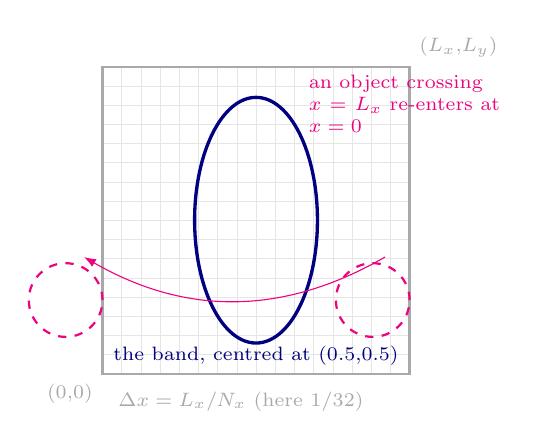
\begin{tikzpicture}[scale=0.78,font=\scriptsize]
  \draw[step=0.3125,LightGray!60,very thin] (0,0) grid (5,5);
  \draw[DarkGray,thick] (0,0) rectangle (5,5);
  \node[anchor=north east,DarkGray] at (0,0) {(0,0)};
  \node[anchor=south west,DarkGray] at (5,5) {($L_x$,$L_y$)};
  \draw[NavyBlue,very thick] (2.5,2.5) ellipse (1.0 and 2.0);
  \node[NavyBlue] at (2.5,0.3) {the band, centred at (0.5,0.5)};
  \draw[RubineRed,thick,dashed] (4.4,1.2) circle (0.6);
  \draw[RubineRed,thick,dashed] (-0.6,1.2) circle (0.6);
  \draw[-{Latex[length=1.5mm]},RubineRed] (4.6,1.9) to[bend left] (-0.3,1.9);
  \node[RubineRed,anchor=west,text width=2.6cm] at (3.2,4.4) {an object crossing $x = L_x$ re-enters at $x = 0$};
  \node[DarkGray,anchor=west] at (0.1,-0.45) {$\Delta x = L_x/N_x$ (here $1/32$)};
\end{tikzpicture}
\end{columns}
\end{frame}

\begin{frame}{The delta function}
\label{fr:delta}
\begin{columns}[T]
\column{0.42\textwidth}
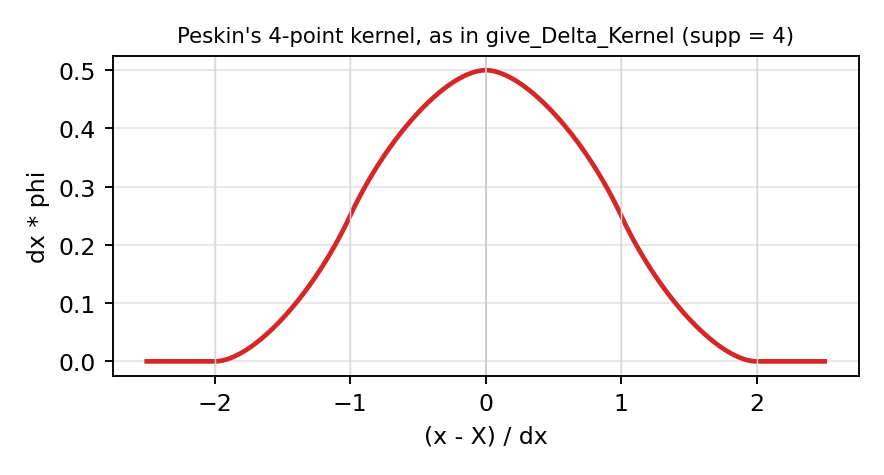
\includegraphics[width=\textwidth]{ch4a-delta.png}
\column{0.56\textwidth}
\footnotesize
\code{give\_Delta\_Kernel}: Peskin's 4-point function,
\begin{align*}
\phi(r) &= \tfrac{1}{8}\big(3 - 2|r| + \sqrt{1 + 4|r| - 4r^2}\big), & |r| &< 1,\\
\phi(r) &= \tfrac{1}{8}\big(5 - 2|r| - \sqrt{-7 + 12|r| - 4r^2}\big), & 1 \le |r| &< 2,
\end{align*}
zero beyond; $\delta_h(\mathbf{x}) = \phi(x/\Delta x)\,\phi(y/\Delta y)/(\Delta x \Delta y)$. \code{supp = 4} is its width in cells.
\begin{itemize}
  \item The force of a point is spread over the $4 \times 4$ cells around it, and its velocity is averaged from them: the boundary is a layer about two cells thick.
  \item The weights of the four cells sum to one wherever the point sits (checked for the kernel above).
\end{itemize}
\end{columns}
\end{frame}

\begin{frame}{How far apart the points should be}
\label{fr:spacing}
\small
\begin{itemize}
  \item Points farther apart than about $\Delta x$ leave gaps the fluid leaks through; much closer than $\Delta x/2$ buys nothing. The rule of Lecture 2: \al{$\Delta s \approx \Delta x/2$}.
  \item The rubber-band generator takes $N = 2 N_x$ points, which is right on average, but spaces them evenly in angle on an ellipse: $\Delta s$ runs from $0.63\,\Delta x$ at the ends of the long axis to $1.25\,\Delta x$ at the sides (slide \ref{fr:vertexpic}). Space points by arc length when you write your own (chapter 4c), and print $\Delta s$ from the \code{.vertex} file (the differences of consecutive points, three lines in either language) next to $\Delta x$.
  \item Chapter 5 says why (the discrete delta function and its moment conditions); chapter 4d shows what the spacing does to the results.
  \item The same rule holds for IBAMR's fibre structures ($\Delta s = \Delta x/2$) and differs for IBFE meshes ($\Delta s \approx \Delta x$): Lecture 2's one-line summary, chapter 18 for the finite-element side.
\end{itemize}
\end{frame}

% ---------------------------------------------------------------- structure files
\begin{frame}{The structure files: one name, many extensions (1/2)}
\label{fr:family}
\scriptsize
\begin{tabular}{@{}L{0.13\textwidth}L{0.16\textwidth}L{0.38\textwidth}L{0.18\textwidth}@{}}
\toprule
File & Flag & Columns after the count line & Slide \\
\midrule
\code{.vertex} & always read & \code{x y} per point & \ref{fr:vertex} \\
\code{.spring} & \code{springs} & \code{i j k L [alpha]} & \ref{fr:spring} \\
\code{.d\_spring} & \code{damped\_springs} & \code{i j k L b} & \ref{fr:dspring} \\
\code{.beam} & \code{beams} & \code{i j k k\_b C} & \ref{fr:beam} \\
\code{.nonInv\_beam} & \code{nonInvariant\_beams} & \code{i j k k\_b Cx Cy} & \ref{fr:noninv} \\
\code{.target} & \code{target\_pts} & \code{i k\_t} & \ref{fr:target} \\
\code{.mass} & \code{mass\_pts} & \code{i k\_m m} & \ref{fr:mass} \\
\code{.muscle} & \code{FV\_LT\_muscle} & \code{i j LFO SK a b Fmax} & \ref{fr:others} \\
\code{.3\_muscle} & \code{3\_element\_muscle} & \code{i j LFO SK a b Fmax kSpr alpha} (Python reads \code{.muscle}) & \ref{fr:others} \\
\bottomrule
\end{tabular}

\vspace{1mm}
\small Every file in this table starts with one line holding the number of entries, then one entry per line, space-separated, written with \code{\%1.16e}. The counts are read but the readers take every line that follows, so the count must match. \code{i}, \code{j}, \code{k} are point indices in the order of the \code{.vertex} file.
\end{frame}

\begin{frame}{The structure files: one name, many extensions (2/2)}
\label{fr:family2}
\scriptsize
\begin{tabular}{@{}L{0.14\textwidth}L{0.16\textwidth}L{0.46\textwidth}L{0.14\textwidth}@{}}
\toprule
File & Flag & Layout & Slide \\
\midrule
\code{.porous} & \code{porous\_media} & count, then \code{i alpha flag} & \ref{fr:others} \\
\code{.poroelastic} & \code{poroelastic} & count, then \code{i alpha} & \ref{fr:others} \\
\code{.tracer} & \code{tracers} & count, then \code{x y} per tracer & \ref{fr:others} \\
\code{.concentration} & \code{concentration} & an $N_y \times N_x$ array of values, no count line & \ref{fr:others2} \\
\code{.brinkman} & \code{brinkman} & the same layout & \ref{fr:others2} \\
\code{.user\_force} & \code{user\_force\_model} & one header line, then whatever your force function reads & \ref{fr:others2} \\
\code{.coagulation} & \code{coagulation} & one value per line: start index, radius, force threshold, cell sizes & \ref{fr:others2} \\
\code{.geo\_connect} & read if present & \code{i j} pairs, no count line: geometric connections for the force and source routines & \ref{fr:others2} \\
\bottomrule
\end{tabular}

\vspace{1mm}
\small A flag set to 1 without its file stops the run (the reader cannot open the file); a file without its flag is ignored. All of them are read once, at the start; the \code{update\_*} functions of chapter 4c change the arrays in memory, not the files.
\end{frame}

\begin{frame}[fragile]{\code{.vertex}: the points}
\label{fr:vertex}
\begin{columns}[T]
\column{0.46\textwidth}
\begin{lstlisting}[style=plain]
64
6.9999999999999996e-01 5.0000000000000000e-01
6.9903694533443939e-01 5.3920685613182429e-01
6.9615705608064604e-01 5.7803612880645128e-01
...
\end{lstlisting}
\small The shipped \code{rubberband.vertex}: 64 points on an ellipse centred at (0.5, 0.5) with semi-axes 0.2 ($x$) and 0.4 ($y$), starting at the rightmost point and going counter-clockwise.
\column{0.52\textwidth}
\small
\begin{itemize}
  \item Line 1: the number of points $N$. Then $N$ lines of \code{x y}, in metres or whatever unit the grid uses.
  \item The order is the point index used by every other file: the first point is 0 in Python, 1 in MATLAB (slide \ref{fr:index}).
  \item Several boundaries go into \al{one list}: two plates of 100 points are points 1--100 and 101--200 (MATLAB), and you keep track of where one ends (Lecture 2). IBAMR takes one \code{.vertex} per structure instead (chapter 6).
  \item The reader takes \code{\%f \%f} pairs: no comments, no blank lines, no third column.
\end{itemize}
\end{columns}
\end{frame}

\begin{frame}{The example's points on the grid}
\label{fr:vertexpic}
\begin{center}
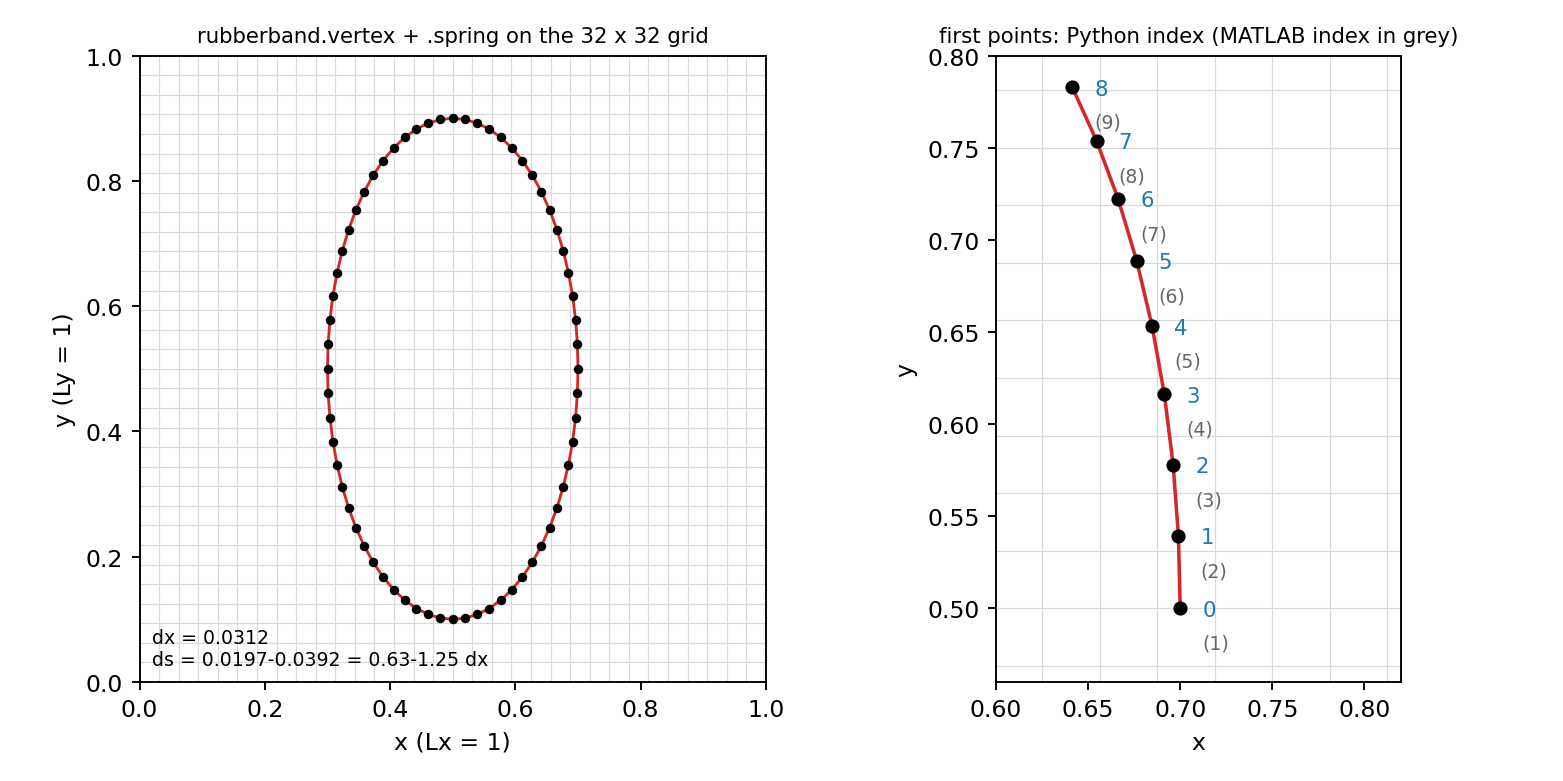
\includegraphics[width=0.78\textwidth]{ch4a-rubberband-geometry.png}
\end{center}
\small The 64 points on the $32 \times 32$ grid (left; the red segments are the \code{.spring} entries) and the first nine with both numberings (right: Python's in blue, MATLAB's in grey). The spacing is uneven because the generator spaces the points in angle, not in arc length (slide \ref{fr:spacing}).
\end{frame}

\begin{frame}[fragile]{Indices: MATLAB counts from 1, Python from 0}
\label{fr:index}
\begin{columns}[T]
\column{0.5\textwidth}
\small
The same example, the shipped \code{rubberband.spring}:
\begin{lstlisting}[style=plain]
matIB2d (1-based)          pyIB2d (0-based)
64                         64
1 2 2.5e+04 0.0e+00        0 1 2.5e+04 0.0e+00
2 3 2.5e+04 0.0e+00        1 2 2.5e+04 0.0e+00
...                        ...
63 64 2.5e+04 0.0e+00      62 63 2.5e+04 0.0e+00
64 1 2.5e+04 0.0e+00       63 0 2.5e+04 0.0e+00
\end{lstlisting}
(values abbreviated). The same holds for \code{.beam}, \code{.d\_spring} and \code{.target}: \code{Wobbly\_Beam} tethers points \code{0} and \code{63} in Python; the MATLAB generators write \code{s} for \code{s = 1:N}.
\column{0.48\textwidth}
\small
\begin{itemize}
  \item Both readers use the numbers as they are: MATLAB indexes \code{xLag(i)}, Python \code{xLag[i]}. Neither shifts.
  \item So a structure file written for one version is \al{off by one} in the other: in MATLAB an index 0 is an error (``Index exceeds \ldots'' or ``Array indices must be positive integers''); in Python an index $N$ is an \code{IndexError}, and an index 1 where 0 was meant silently connects the wrong points.
\end{itemize}
\end{columns}
\end{frame}

\begin{frame}{Indices, continued: porting between the versions}
\label{fr:index2}
\small
\begin{itemize}
  \item IBAMR counts from 0, like Python (chapter 6, which has the same warning the other way round). MeshmerizeMe writes both (chapter 4f).
  \item When you port an example, convert the files, not the reader: \code{i - 1} on every index column (or \code{+ 1} the other way), in a script, and re-run the geometry checker (slide \ref{fr:check}).
  \item The count line and the value columns do not change; only the index columns do: 2 of them in \code{.spring} and \code{.d\_spring}, 3 in the beam files, 1 in \code{.target}, \code{.mass}, \code{.porous}, \code{.poroelastic}, 2 in \code{.muscle} and \code{.geo\_connect}.
  \item The output does not care: the VTK files number points from 0 in both versions (VTK's convention), which is one more reason to check the structure in the output's first dump rather than in the input files.
\end{itemize}
\begin{punchbox}
\small The 2024 ``Introduction to IB2D'' deck shows the MATLAB numbering (``vertex 1 \ldots N''); Lecture 9 and Lecture 2 (2022) show \code{x\_0 \ldots x\_\{N-1\}}. Both are right, for their version.
\end{punchbox}
\end{frame}

\begin{frame}[fragile]{\code{.spring}: two points, a stiffness, a resting length, an exponent}
\label{fr:spring}
\begin{columns}[T]
\column{0.46\textwidth}
\begin{lstlisting}[style=plain]
64                      # number of springs
1 2 2.5e+04 0.0e+00     # i j k L  (MATLAB indices)
2 3 2.5e+04 0.0e+00
...
64 1 2.5e+04 0.0e+00    # closes the band
\end{lstlisting}
\footnotesize
The force on point $i$ from the spring to $j$, with $\mathbf{d} = \mathbf{X}_j - \mathbf{X}_i$:
\[
\mathbf{F}_i = \tfrac{1}{2}(\alpha + 1)\, k\, \big(|\mathbf{d}| - L\big)^{\alpha}\, \frac{\mathbf{d}}{|\mathbf{d}|},
\]
and $\mathbf{F}_j = -\mathbf{F}_i$; so $\alpha = 1$ is Hooke's law $k(|\mathbf{d}| - L)$ (\code{give\_Me\_Spring\_Lagrangian\_Force\_Densities}).
\column{0.52\textwidth}
\small
\begin{itemize}
  \item Columns: \code{i j k L} and an optional fifth, \code{alpha}, the degree of nonlinearity. Missing: 1 (linear). MATLAB's \code{textscan} returns \code{NaN} for a missing fifth value and the reader fills 1 (a four-column file works as shipped); the Python reader accepts \code{NaN}/\code{NA}/\code{NULL} markers and fills 1, and stops with a message if rows have different lengths.
  \item \code{L = 0} (this example) makes a band that wants to shrink to a point; the fluid inside resists, and the band settles near a circle of the enclosed area. \code{L = ds} (the generator of Lecture 9) makes a band at rest in its initial length.
\end{itemize}
\end{columns}
\end{frame}

\begin{frame}{Springs, continued}
\label{fr:spring2}
\small
\begin{itemize}
  \item Any network is allowed: no limit on springs per point, diagonals, cross-links. A spring over the periodic edge is handled inside the force routine (a separation longer than half the box is shortened by $L_x$ or $L_y$); only the beams have a named check function.
  \item Units: \code{k} is a force per length of stretch (N/m), per Lagrangian point; the spreading multiplies by $\Delta s$. The convention $\kappa\, \Delta s/\Delta s^2$ of Lecture 9's generator makes the stiffness independent of the resolution; chapters 6 and 8b discuss the scaling.
  \item \code{NL\_Rubberband\_With\_Springs} is the same band with \code{alpha = 2} and $k = 10^5$: the force grows with the square of the stretch, a rubber that stiffens.
  \item With \code{update\_springs = 1}, \code{update\_Springs(dt, current\_time, xLag, yLag, springs\_info)} is called every step and returns the spring table, so $k$ and $L$ can change in time: the heart-tube examples pump by changing resting lengths (chapters 4c and 4e).
\end{itemize}
\end{frame}

\begin{frame}[fragile]{\code{.d\_spring}: damped springs}
\label{fr:dspring}
\begin{columns}[T]
\column{0.46\textwidth}
\begin{lstlisting}[style=plain]
64
1 2 2.5e+04 0.0e+00 5.0e+00    # i j k L b
2 3 2.5e+04 0.0e+00 5.0e+00
...
\end{lstlisting}
\small
\[
\mathbf{F}_i = k\, (|\mathbf{d}| - L)\, \frac{\mathbf{d}}{|\mathbf{d}|} - b\, \mathbf{U}_i, \qquad \mathbf{F}_j = -\mathbf{F}_i ,
\]
with $\mathbf{U}_i$ the leader point's own velocity, taken as its displacement since the previous step over $\Delta t$ (the driver keeps \code{xLag\_P}, \code{yLag\_P} for this); linear only, and the damping is of the first point's motion, not of the relative motion of the pair (both versions).
\column{0.52\textwidth}
\small
\begin{itemize}
  \item Flag \code{damped\_springs = 1}; the file \code{<name>.d\_spring}; five columns, all required.
  \item \code{Rubberband\_with\_Damped\_Springs} is the springs example with $b = 5$: the band relaxes the same way (slide \ref{fr:relax}); at $b = 5$ the two curves are indistinguishable.
  \item A damped spring is the simplest way to stop a structure ringing when the stiffness has to be high; \code{update\_damp\_springs} can change $k$, $L$ and $b$ in time (chapter 4c).
  \item Added in Reloaded (2017); not in IBAMR's file set (IBAMR's target points have the damping parameter instead: chapter 6).
\end{itemize}
\end{columns}
\end{frame}

\begin{frame}[fragile]{\code{.beam}: torsional springs over three points}
\label{fr:beam}
\begin{columns}[T]
\column{0.5\textwidth}
\begin{lstlisting}[style=plain]
62                                   # Wobbly_Beam (Python)
0 1 2 7.5e+09 0.0e+00                # i j k  k_b  C
1 2 3 7.5e+09 0.0e+00
...
249                                  # Rubberband_with_Beams
248 0 1 1.0e+07 -1.2851754376167265e-06
0 1 2 1.0e+07 -1.2851754376155979e-06
\end{lstlisting}
\column{0.48\textwidth}
\footnotesize
With $\mathbf{p}, \mathbf{q}, \mathbf{r}$ the three points (left, middle, right):
\[
c = (x_r - x_q)(y_q - y_p) - (y_r - y_q)(x_q - x_p),
\]
the cross product of the two segments, a signed area; $C$ is its rest value. The three forces are $k_b\,(c - C)$ times the perpendiculars of the segments, with the signs as coded:
\begin{align*}
\mathbf{F}_p &= k_b (c - C)\, \big(y_r - y_q,\; -(x_r - x_q)\big),\\
\mathbf{F}_r &= k_b (c - C)\, \big(y_q - y_p,\; -(x_q - x_p)\big),\\
\mathbf{F}_q &= k_b (c - C)\, \big(y_r - y_p,\; -(x_r - x_p)\big) = \mathbf{F}_p + \mathbf{F}_r
\end{align*}
(\code{give\_Me\_Beam\_Lagrangian\_Force\_Densities}; the three do not sum to zero, unlike the gradient of a bending energy, which would give the end forces the opposite sign).
\end{columns}
\end{frame}

\begin{frame}{Torsional springs, continued}
\label{fr:beam2}
\small
\begin{itemize}
  \item Columns: \code{i j k} (left, middle, right), \code{k\_b}, \code{C}. The force acts on all three; the code's comment ``force is exerted on the middle point'' names where it is applied in the bookkeeping.
  \item \code{C = 0} is a straight beam at rest (\code{Wobbly\_Beam}: a beam whose ends are target points, bending back after an initial curve). The rubber band's file gives one constant \code{C} $= -1.285 \cdot 10^{-6}$ to all 249 beams (its generator computes the curvatures of a second, rounder geometry), while the cross products of its initial ellipse range from $-4.8 \cdot 10^{-6}$ to $-3 \cdot 10^{-8}$: the band is not at rest and relaxes towards a rounded shape. The 2024 deck's ``preferred curvature'' is this number, in units of length$^2$, not $1/$length.
  \item The model is \al{invariant under rotation} (a rotated beam feels no force), unlike the non-invariant beam of the next slide. It is weak against pure stretching, so beams are usually combined with springs.
  \item A beam cannot start or end at the ends of an open structure: $N - 2$ beams for $N$ points in a line, $N$ for a closed loop. The generator writes one line per interior point.
  \item IBAMR's \code{.beam} is the non-invariant kind with a curvature vector (chapter 6, chapter 10).
\end{itemize}
\end{frame}

\begin{frame}[fragile]{\code{.nonInv\_beam}: the beam equation with a rest curvature vector}
\label{fr:noninv}
\begin{columns}[T]
\column{0.52\textwidth}
\begin{lstlisting}[style=plain]
N_beams
i j k  k_b  Cx  Cy        # six columns
...
\end{lstlisting}
\footnotesize
\begin{align*}
\mathbf{F}_q &= 2 k_b\,(\mathbf{X}_r - 2\mathbf{X}_q + \mathbf{X}_p - \mathbf{C}),\\
\mathbf{F}_p &= \mathbf{F}_r = -\tfrac{1}{2}\mathbf{F}_q ,
\end{align*}
the discrete fourth derivative of the 2024 deck's $\mathbf{F} = k_{NIB}\, \partial^4 (\mathbf{X} - \mathbf{X}_b)/\partial s^4$ assembled from second differences (\code{give\_Me\_nonInv\_Beam\_Lagrangian\_Force\_Densities}).
\column{0.46\textwidth}
\footnotesize
\begin{itemize}
  \item Flag \code{nonInvariant\_beams = 1}, file \code{<name>.nonInv\_beam}, six columns: the rest ``curvature'' is the vector $\mathbf{C} = (C_x, C_y)$ of second differences of the preferred shape.
  \item \al{Non-invariant}: the force depends on the orientation of the structure, so a rotated beam is bent back towards its original orientation. Right for a structure clamped in space (a flag, a leaf on a stem: \code{Wobbly\_NonInv\_Beam}); wrong for a free swimmer, which needs the torsional beam.
  \item Same convention as IBAMR's beams and its \code{Cx Cy} columns (chapter 10), which is why a non-invariant beam file converts to IBAMR by shifting the indices.
  \item Added in Reloaded (2017), with the explanation quoted in the 2021--24 decks.
\end{itemize}
\end{columns}
\end{frame}

\begin{frame}[fragile]{\code{.target}: tethered points}
\label{fr:target}
\begin{columns}[T]
\column{0.46\textwidth}
\begin{lstlisting}[style=plain]
2                      # Wobbly_Beam: the two ends
0 2.0e+08              # i  k_t
63 2.0e+08
6552                   # the sawtooth channel (chapter 4c)
1 1.0e+11
2 1.0e+11
...
\end{lstlisting}
\footnotesize
\[
\mathbf{F}_i = k_t\,\big(\mathbf{X}^{\mathrm{target}}_i - \mathbf{X}_i\big),
\]
a zero-rest-length spring to a position that is, by default, the point's initial position (\code{give\_Me\_Target\_Lagrangian\_Force\_Densities}).
\column{0.52\textwidth}
\small
\begin{itemize}
  \item Two columns: the point index and its stiffness. Any subset of the points; a point can be a target point and a spring end at once.
  \item Target points are how IB2d holds a structure in place (the beam's clamped ends, channel walls, a cylinder) and how it \al{prescribes motion}: with \code{update\_target = 1} your \code{update\_Target\_Point\_Positions} moves the target positions every step and the points follow (chapter 4c's sawtooth: $10^{11}$ for 6552 wall points).
\end{itemize}
\end{columns}
\end{frame}

\begin{frame}{Target points, continued}
\label{fr:target2}
\small
\begin{itemize}
  \item The stiffness is a penalty: too small and the points lag behind their targets (a leaky wall), too large and $\Delta t$ must shrink (chapter 4d). Start from the examples' values and the grid they use.
  \item The target positions are kept in the driver's \code{target\_info} array (columns: index, $x$, $y$, $k_t$), which is what the update function edits (Lecture 11): a target point's position is a number in memory, not a point of the \code{.vertex} file, so moving it costs nothing.
  \item A rigid object in IB2d is a closed curve of target points; a wall is a line of them; a hinge is a target point at one end of a beam. IBAMR's \code{.target} adds a damping coefficient (chapter 6) and chapter 9a has the same lesson for IBAMR.
\end{itemize}
\end{frame}

\begin{frame}[fragile]{\code{.mass}: massive points and gravity}
\label{fr:mass}
\begin{columns}[T]
\column{0.46\textwidth}
\begin{lstlisting}[style=plain]
N_mass
i  k_m  m           # index, mass-spring stiffness, mass
...
\end{lstlisting}
\footnotesize
Each massive point is a \al{separate particle} of mass $m$ at $\mathbf{Y}_i$, tied to the boundary point by a stiff spring:
\begin{align*}
\mathbf{F}_i &= k_m\,(\mathbf{Y}_i - \mathbf{X}_i),\\
m\,\ddot{\mathbf{Y}}_i &= -\mathbf{F}_i + m\,\mathbf{g},
\end{align*}
integrated by the driver (\code{please\_Move\_Massive\_Boundary}, \code{please\_Update\_Massive\_Boundary\_Velocity}); the boundary point itself still moves with the fluid.
\column{0.52\textwidth}
\small
\begin{itemize}
  \item Flags \code{mass\_pts = 1}, and \code{gravity = 1} with \code{x\_gravity\_vec\_comp}, \code{y\_gravity\_vec\_comp} giving the direction (the examples use $(0, -1)$); the magnitude $g = 9.80665$ is hard-coded in the velocity update of the massive points.
  \item This is the penalty-IB idea (chapter 13 for IBAMR): the IB point is massless, the inertia sits in its shadow particle. The spring stiffness $k_m$ must be high enough that the two stay together, which again limits $\Delta t$.
  \item Uses: sinking cells, ``massive cells racing'' under gravity vs. flow (\code{Example\_Mass\_Points}, \code{Gravity\_Cellular\_Race}), flexible structures with inertia.
  \item IBAMR's \code{.mass} has the same three numbers in a different order (\code{i mass kappa}): chapter 6.
\end{itemize}
\end{columns}
\end{frame}

\begin{frame}{The other files, briefly (1/2)}
\label{fr:others}
\small
\begin{itemize}
  \item \al{\code{.muscle}} (\code{FV\_LT\_muscle}): \code{i j LFO SK a b Fmax}: a muscle between two points, with the length of maximal tension \code{LFO}, a length-tension width \code{SK}, the Hill force-velocity constants \code{a}, \code{b}, and the peak force \code{Fmax}; activation comes from a function you write (chapter 4e; the 2015 paper).
  \item \al{\code{.3\_muscle}} (\code{3\_element\_muscle}): the seven above plus a parallel nonlinear spring \code{kSpr}, \code{alpha}. MATLAB reads \code{<name>.3\_muscle}; the Python port reads \code{<name>.muscle} for it and marks it untested.
  \item \al{\code{.porous}} (\code{porous\_media}): \code{i alpha flag}: a porosity coefficient per point and a stencil flag; the points slip through the fluid in proportion to the force on them (\code{please\_Compute\_Porous\_Slip\_Velocity}). \al{\code{.poroelastic}} (\code{poroelastic}): \code{i alpha}, the Brinkman-type solid of Reloaded.
  \item \al{\code{.tracer}} (\code{tracers}): a count line, then \code{x y} per passive tracer; they move with the fluid and are written as \code{tracer.NNNN.vtk}.
\end{itemize}
\end{frame}

\begin{frame}{The other files, briefly (2/2)}
\label{fr:others2}
\small
\begin{itemize}
  \item \al{\code{.concentration}} (\code{concentration}): the initial scalar field as an $N_y \times N_x$ array of numbers (the reader builds a format of $N_x$ floats per line); \al{\code{.brinkman}} (\code{brinkman}): the permeability field in the same layout.
  \item \al{\code{.user\_force}} (\code{user\_force\_model}): one header line, then whatever your \code{give\_Me\_General\_User\_Defined\_Force\_Densities} expects (MATLAB reads it with \code{importdata}).
  \item \al{\code{.coagulation}} (\code{coagulation}): one number per line: the first index of the coagulating cells, a threshold radius, a threshold force, then the number of points in each cell.
  \item \al{\code{.geo\_connect}}: \code{i j} pairs, without a count line, read whenever the file exists; the driver passes them to the force routines (the coagulation model and the concentration source use them). The output's connection file follows the springs, not this file.
\end{itemize}
Chapter 4e shows the muscle, porous and tracer examples; chapter 4c the update functions.
\end{frame}

\begin{frame}{IB2d and IBAMR files, the short version (1/2)}
\label{fr:ibamr}
\small
Chapter 6 has the full comparison table; the points that matter when you move a structure between the two:
\begin{itemize}
  \item \al{Index base}: IB2d/MATLAB 1, IB2d/Python 0, IBAMR 0.
  \item \al{Several structures}: one list in IB2d; one set of files per structure in IBAMR (\code{structure\_names} in \code{input2d}).
  \item \al{Springs}: IB2d \code{i j k L [alpha]}; IBAMR \code{i j kappa L [fcn\_idx [params]]}, the force function chosen by an index, not an exponent.
  \item \al{Beams}: IB2d's \code{.beam} is a torsional spring with a scalar \code{C}; IBAMR's \code{.beam} is IB2d's \code{.nonInv\_beam} with \code{Cx Cy} (chapter 10).
\end{itemize}
\end{frame}

\begin{frame}{IB2d and IBAMR files, the short version (2/2)}
\label{fr:ibamr2}
\small
\begin{itemize}
  \item \al{Target points}: IB2d \code{i k\_t}; IBAMR \code{i kappa [eta]} with an optional damping; \al{mass}: IB2d \code{i k\_m m}, IBAMR \code{i m kappa}.
  \item IBAMR only: \code{.xspring}, \code{.anchor}, \code{.rod}, \code{.director}, \code{.inst}, \code{.source}; IB2d only: \code{.d\_spring}, \code{.muscle}, \code{.porous}, \code{.poroelastic}, \code{.tracer}, \code{.concentration}, \code{.user\_force}, \code{.coagulation}, \code{.geo\_connect}.
  \item \al{Domain}: IB2d's box starts at the origin and is periodic; IBAMR's goes anywhere, with wall and inflow conditions (chapter 7).
  \item \al{Units}: IB2d's examples are dimensionless in practice; IBAMR's examples mix. Chapter 8b.
\end{itemize}
Lecture 2's rubber-band generator writes both kinds from one script (a flag for the index base); MeshmerizeMe does the same from a drawing (chapter 4f).
\end{frame}

% ---------------------------------------------------------------- generator and checks
\begin{frame}[fragile]{The generator script: \code{Rubberband.m} / \code{Rubberband.py}}
\label{fr:generator}
\begin{columns}[T]
\column{0.5\textwidth}
\begin{lstlisting}[style=plain]
% Grid Parameters (MAKE SURE MATCHES IN input2d !!!)
Nx = 32;  Ny = 32;  Lx = 1.0;  Ly = 1.0;
N = 2*Nx;        % Number of Lagrangian Pts. (2x resolution)
a = 0.4;  b = 0.2;        % semi-axes
ds_Rest = 0;              % Resting length of springs
struct_name = 'rubberband';
[xLag,yLag] = give_Me_Immsersed_Boundary_Geometry(N,a,b);
plot(xLag,yLag,'r-'); hold on; plot(xLag,yLag,'*');
print_Lagrangian_Vertices(xLag,yLag,struct_name);
k_Spring = 2.5e4;
print_Lagrangian_Springs(xLag,yLag,k_Spring,ds_Rest,struct_name);
\end{lstlisting}
\column{0.48\textwidth}
\begin{lstlisting}[style=plain]
function print_Lagrangian_Springs(xLag,yLag,k_Spring,ds_Rest,struct_name)
    N = length(xLag);
    spring_fid = fopen([struct_name '.spring'], 'w');
    fprintf(spring_fid, '%d\n', N );
    for s = 1:N
        if s < N
            fprintf(spring_fid, '%d %d %1.16e %1.16e\n', s, s+1, k_Spring, ds_Rest);
        else
            fprintf(spring_fid, '%d %d %1.16e %1.16e\n', s, 1,   k_Spring, ds_Rest);
        end
    end
    fclose(spring_fid);
\end{lstlisting}
\end{columns}
\small The top of the MATLAB script (left) and its spring writer (right); the Python twin writes the same files with \code{range(N)}: \code{s, s+1} and the closing \code{N-1, 0}, the 0-based files of slide \ref{fr:index}.
\end{frame}

\begin{frame}{The generator: how to use it}
\label{fr:generator2}
\small
\begin{itemize}
  \item The script knows the grid only to choose $N$; it is \al{not called by the run}, and \code{input2d} does not read it. Change either and keep them consistent by hand (Lecture 2: ``if you change the generate\_mesh file, you must run it'').
  \item \code{give\_Me\_Immsersed\_Boundary\_Geometry} (sic) puts $N$ points at equal angles on the ellipse centred at (0.5, 0.5). Write your own geometry function in any language; the files are plain text (Lecture 2 names Python, Julia and Excel on two of its slides).
  \item The same pattern writes \code{.beam} (one line per interior point, \code{s-1 s s+1}), \code{.target} (\code{s k}) and the rest: the example generators are the templates (chapter 4c builds one from scratch).
  \item Write the numbers with full precision (\code{\%1.16e}, as the generators do): a point list rounded to four decimals at $\Delta x = 1/512$ has visible kinks.
  \item Keep the plot the generator draws: it is the first check of the geometry, and chapter 4c's exercise starts from it.
\end{itemize}
\end{frame}

\begin{frame}{Check the geometry before you run}
\label{fr:check}
\small
\begin{itemize}
  \item \al{\code{test\_IB2d\_IBAMR\_Geometry.m}} (Appendix A; \code{examples/support/matlab-exercises} in this repository, with its Python version \code{test\_ib\_geometry.py}): reads a \code{.vertex} and a \code{.spring} file and makes two figures: the points with their index labels, and the points with the spring connections (alternating colours, so a missing or doubled spring stands out). Two lines to set at the top: \code{flag\_IBAMR = 0} for 1-based files (MATLAB IB2d; Lecture 2's \code{test\_IB\_Geometry\_and\_Springs}), 1 for Python IB2d or IBAMR files, which count from 0; and \code{numCols}, the number of columns of the \code{.spring} file. The Python version: \code{python3 test\_ib\_geometry.py NAME [--ibamr]} saves \code{NAME\_points.png} and \code{NAME\_springs.png}.
  \item \al{\code{read\_Vertex\_Points\_and\_Plot\_Them.m}} (the IB2d repository, \code{data\_analysis/analysis\_in\_matlab/DA\_Blackbox}): the vertices only.
  \item Look for: a spring that is missing (the band not closed: a classic off-by-one, chapter 6), a point outside $[0, L_x] \times [0, L_y]$, points closer than $\Delta x/4$ or farther than $\Delta x$ (compute $\Delta s$ from the file; the checker does not), two structures that overlap.
  \item A second check costs nothing: run with \code{Tfinal} set to a few $\Delta t$ and \code{print\_dump = 1}, and open dump 0000 (chapter 4b). The initial frame shows the structure as the code read it, with the connections it will draw.
\end{itemize}
\end{frame}

% ---------------------------------------------------------------- output
\begin{frame}[fragile]{The output: \code{viz\_IB2d/} and \code{hier\_IB2d\_data/}}
\label{fr:output}
\begin{columns}[T]
\column{0.5\textwidth}
\begin{lstlisting}[style=plain]
viz_IB2d/
  lagsPts.0000.vtk        # the points
  lagPtsConnect.0000.vtk  # the points joined along the springs (springs = 1)
  Omega.0000.vtk          # vorticity          (save_Vorticity)
  P.0000.vtk              # pressure           (save_Pressure)
  u.0000.vtk              # velocity vectors   (save_uVec)
  uMag.0000.vtk           # |u|                (save_uMag)
  uX, uY, fX, fY, fMag    # when their flags are 1
  tracer.0000.vtk         # with tracers
  concentration.0000.vtk  # with a concentration
  ... one set per dump: 0001, 0002, ...
hier_IB2d_data/           # with save_hier = 1
  fX_Lag.0000.vtk  fY_Lag.0000.vtk  fMag.0000.vtk
  fNorm, fTan             # normal/tangential (MATLAB, > 5 points)
\end{lstlisting}
\column{0.48\textwidth}
\small
\begin{itemize}
  \item Dump \code{0000} is $t = 0$; then one dump every \code{print\_dump} steps, numbered consecutively: $t = $ dump $\times$ \code{print\_dump} $\times \Delta t$.
  \item 76 dumps of the $32^2$ example: 456 files, 6.7 MB in \code{viz\_IB2d} (Omega 15 KB, u 33 KB, points 3 KB per dump) and 0.9 MB of forces. Text files: the size grows with $N_x N_y$.
  \item With damped springs instead of springs, Python writes no connection file and MATLAB writes \code{damp\_Connect.NNNN.vtk}. MATLAB adds \code{viz\_IB2d/Data\_For\_Restart/} for poroelastic runs.
\end{itemize}
\end{columns}
\end{frame}

\begin{frame}{The output files' format}
\label{fr:output2}
\small
\begin{itemize}
  \item All files are \al{VTK legacy text}. The Python writer with the \code{vtk} module (the runs here) writes ``\# vtk DataFile Version 5.1'' with the \code{OFFSETS}/\code{CONNECTIVITY} cell layout; MATLAB's writers and Python's fallback writer (no \code{vtk} module) write ``Version 2.0'' with the classic \code{CELLS} block. Either way: the fields as \code{STRUCTURED\_POINTS} with \code{DIMENSIONS Nx Ny 1}, \code{SPACING dx dy 1}, \code{ORIGIN 0 0 0} and \code{POINT\_DATA} (\code{SCALARS Omega double}, \code{VECTORS u double}); the points as \code{UNSTRUCTURED\_GRID} with vertex cells (\code{lagsPts}) or line cells (\code{lagPtsConnect}, following the springs); the forces as scalars on those points.
  \item The grid values are on the lattice $x_i = i\,\Delta x$, $i = 0 \ldots N_x - 1$ (no $x = L_x$ column: periodic).
  \item VisIt and ParaView open them directly (chapter 4b: group as \code{Omega.*.vtk}); chapter 33's \code{read\_vtk\_legacy.py/.m} reads them in Python and MATLAB/Octave (it reads both cell layouts); the repository's \code{data\_analysis} folder has IB2d's own readers.
  \item The Python writer uses the \code{vtk} module when it is installed, its own text writer otherwise, with the same layout; the MATLAB writer is its own.
\end{itemize}
\end{frame}

\begin{frame}{A first look at the run}
\label{fr:look}
\begin{center}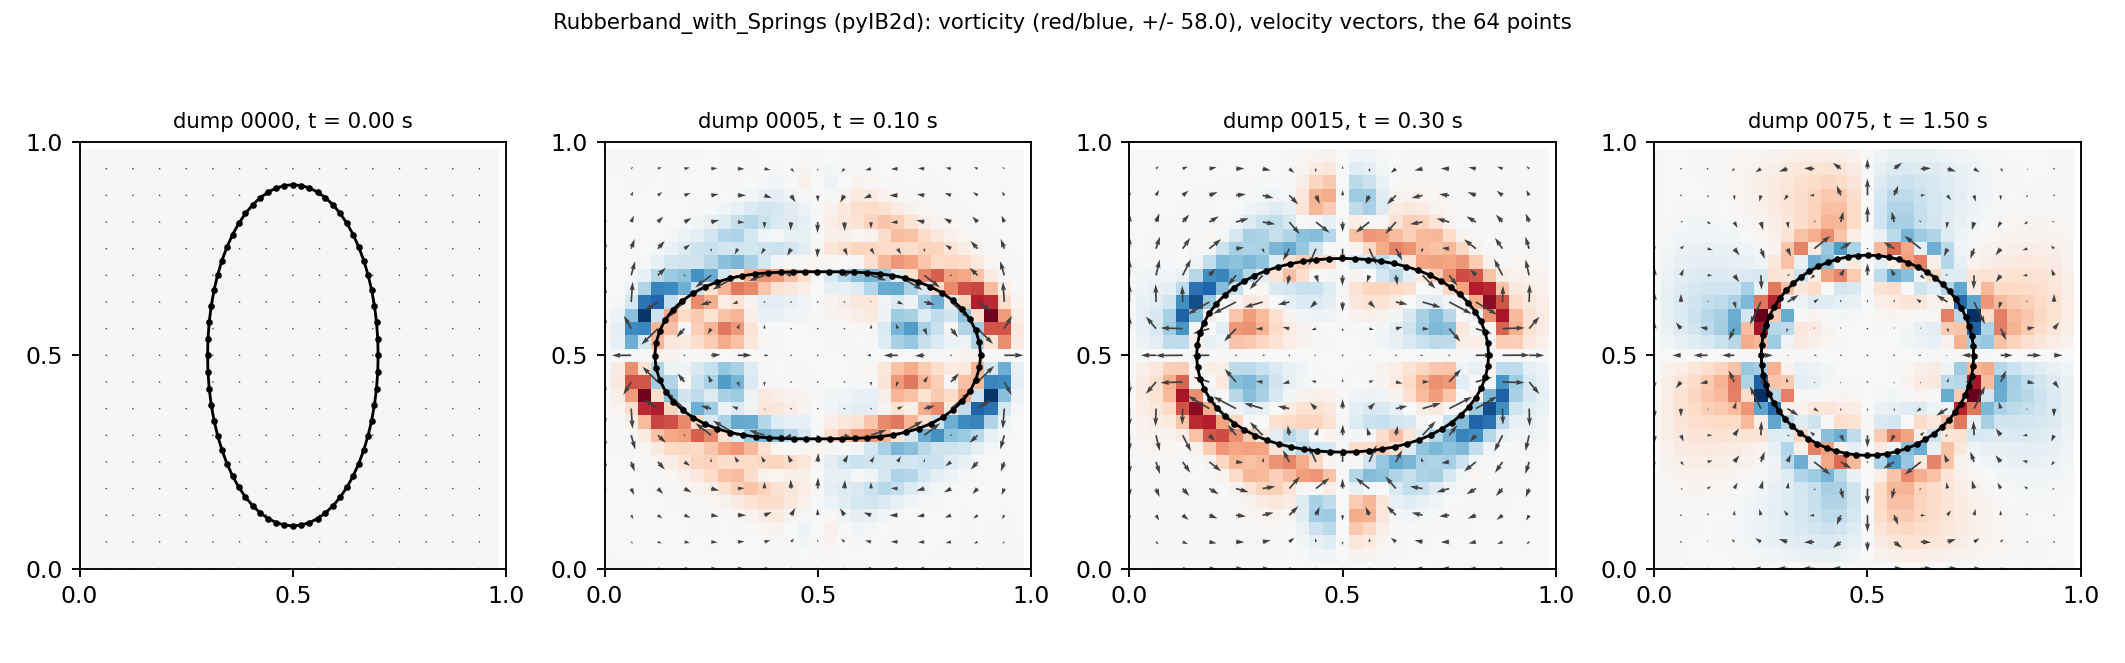
\includegraphics[width=0.96\textwidth]{ch4a-rubberband-frames.png}\end{center}
\footnotesize
\begin{itemize}
  \item The band starts as an ellipse (semi-axes 0.4, 0.2) with zero-rest-length springs; it pulls itself towards a circle, overshoots, and rings down while the fluid it drives spins up four vortices in the corners of the periodic box. Peak speed 4.5 over the run; $\mathrm{Re} = \rho U a/\mu \approx 180$ at most.
  \item Read from the files with chapter 33's reader in a few lines; the pictures of this chapter are matplotlib on the \code{.vtk} files. Chapter 4b does the same in VisIt, with the time slider, and chapter 4d uses this run for the resolution study.
\end{itemize}
\end{frame}

\begin{frame}{Same points, different files}
\label{fr:four}
\begin{center}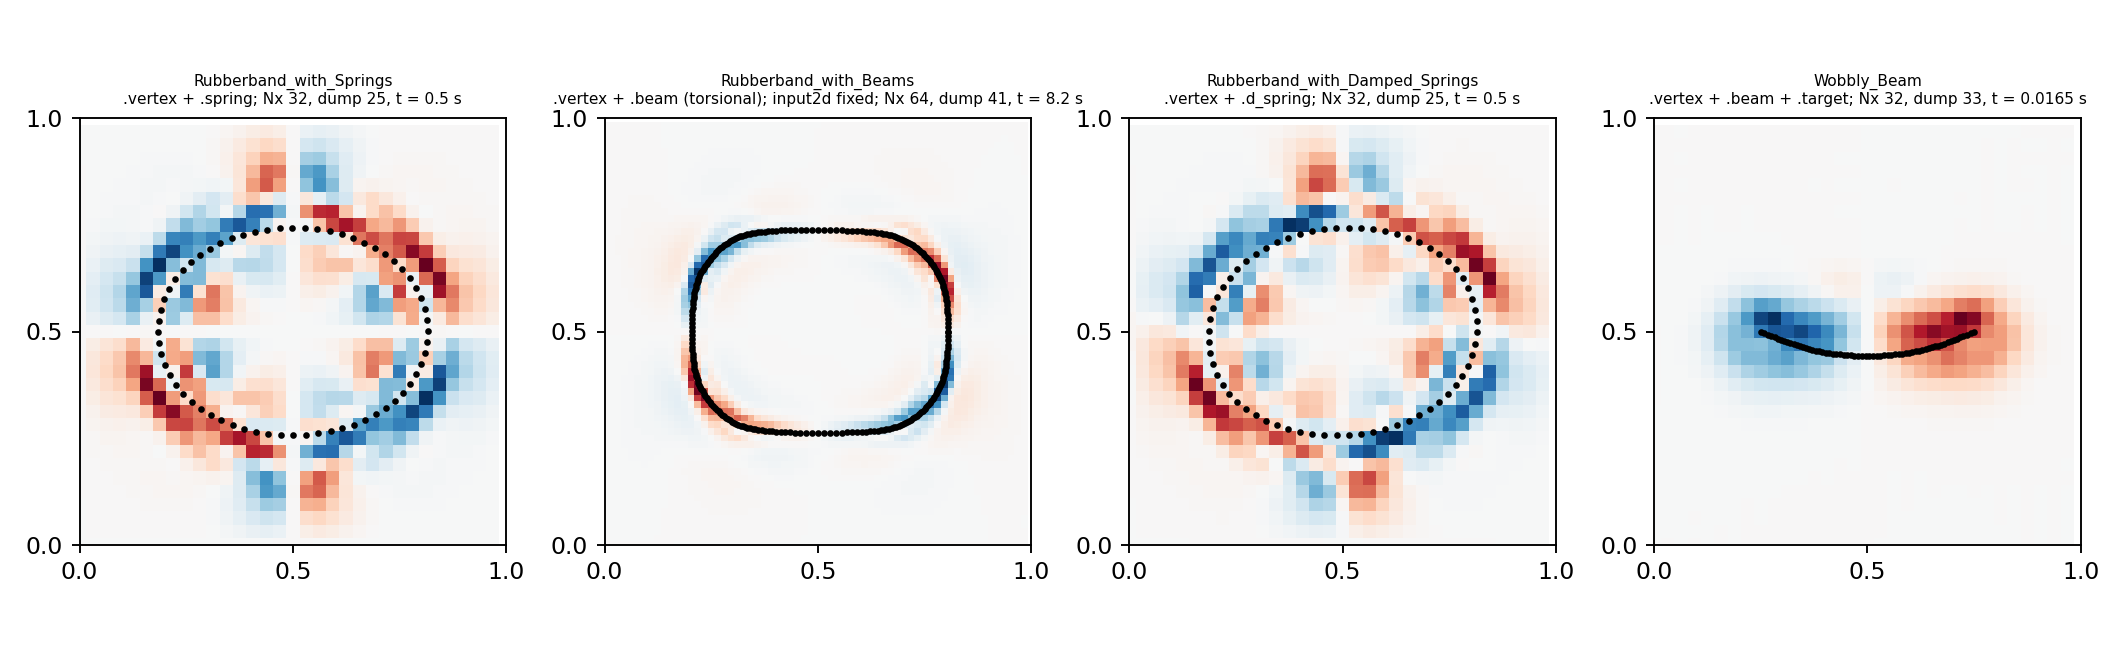
\includegraphics[width=0.9\textwidth]{ch4a-four-examples.png}\end{center}
\footnotesize
\begin{itemize}
  \item Springs, torsional beams, damped springs, and a beam with two target points: the four Python rubber-band examples a third of the way through their runs, vorticity and points. The structure file decides the physics. The springs and damped-springs runs share the 64-point ellipse; the beams example has its own 249-point ellipse with the axes swapped (0.4 along $x$) on a $64^2$ grid; the wobbly beam is a line.
  \item The beams-only band (second panel) moves slowly: its constant rest value $C$ does not match the ellipse (previous slide), so it relaxes towards a rounded square, with $|\mathbf{u}|$ up to 0.26 at $t = 0.4$, $|\omega|$ up to 10 at $t = 0.2$, the half-widths going from 0.40/0.20 to 0.32/0.25, and the vorticity below 1 by $t = 8$ s. That panel is from a corrected \code{input2d}: next slide.
\end{itemize}
\end{frame}

\begin{frame}[fragile]{A trap, found while making the previous picture}
\label{fr:trap}
\small
The shipped \code{pyIB2d/Examples/Rubberband\_with\_Beams/input2d} (2024 clone) has
\begin{lstlisting}[style=input]
beams = 0               % 0 (for no) or 1 (for yes)
update_beams = 0
nonInv_beams = 1        % <-- not a key the code knows
\end{lstlisting}
\begin{itemize}
  \item The parser knows \code{nonInvariant\_beams}, not \code{nonInv\_beams}, and ignores unknown keys. Result: no fibre model at all, ``FIBER MODEL INCLUDES:'' followed by nothing, and 25 s of simulated time in which nothing moves (\code{max |u| = 0} in every dump, 8.6 s of wall time).
  \item The \code{.beam} file has five columns, so the intended flag is \code{beams = 1}; with that the band moves (slide \ref{fr:four}).
  \item Worth a note to the IB2d repository: a one-line fix in the example, and a warning in the parser for unknown keys would catch the whole class of error.
\end{itemize}
\end{frame}

\begin{frame}{What to take from the trap}
\label{fr:trap2}
\small
\begin{itemize}
  \item \al{The console is the check}: every switched-on model is listed under ``FIBER MODEL INCLUDES''. A missing line means a missing or misspelt flag.
  \item A run that produces output is not a run that did what you meant. Open dump 0001 and look for motion.
  \item The flag names are the keys of \code{please\_Initialize\_Simulation} (\code{.m}/\code{.py}); copy them from a working example rather than typing them.
  \item A second copy of a key in the same block does not override the first in Python (the test of slide \ref{fr:parser}): edit the existing line.
\end{itemize}
\begin{punchbox}
\small The same habit serves IBAMR: its input database also accepts keys it never reads and does not warn; the examples print the database into the log with the unused keys marked (chapter 6's log slides). Print or log what the code read, and look at the first frame.
\end{punchbox}
\end{frame}

\begin{frame}{The band relaxes: a number from the output}
\label{fr:relax}
\begin{columns}[T]
\column{0.52\textwidth}
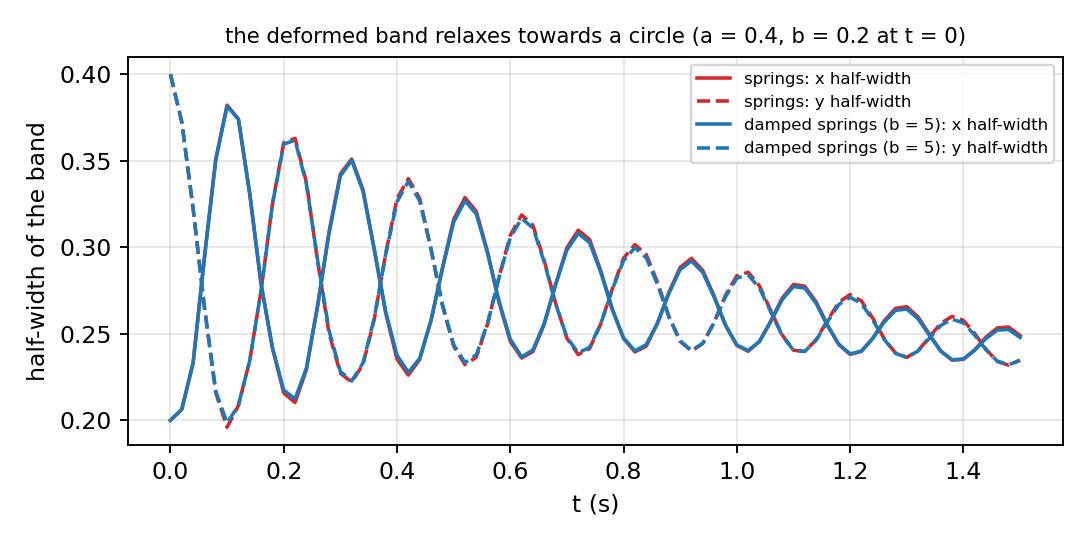
\includegraphics[width=\textwidth]{ch4a-axes-time.png}
\column{0.46\textwidth}
\footnotesize
\begin{itemize}
  \item Half-widths of the point cloud in $x$ and $y$ from \code{lagsPts.NNNN.vtk}: 0.2 and 0.4 at $t = 0$, both near 0.24 by $t = 1.5$ (a circle of about the initial area, $\sqrt{0.2 \cdot 0.4} = 0.28$, less the leak through the 4-cell-thick boundary at this coarse resolution).
  \item With $b = 5$ the damped band's curve lies on the undamped one (differences below 0.002): at this stiffness and resolution the fluid damps the band faster than the dashpots do, and a larger $b$ would be needed to see them.
  \item This is the kind of quantity to track in a study: one number per dump, from the points file, plotted against time and compared across grids (chapter 4d) or stiffnesses. Chapter 33's reader and IB2d's \code{data\_analysis} scripts both do the file reading.
\end{itemize}
\end{columns}
\end{frame}

\begin{frame}{Units and scale}
\label{fr:units}
\small
\begin{itemize}
  \item The comments in \code{input2d} say N s/m$^2$, kg/m$^3$ (one example file says kg/m$^2$) and metres, but the examples are \al{dimensionless in effect}: $\mu = 0.01$, $\rho = 1$, $L = 1$, a band of size 0.4 and stiffness $2.5 \cdot 10^4$ reproduce no particular animal. Treat the numbers as a Reynolds number and a dimensionless stiffness (chapter 8b).
  \item For the rubber band: peak speed about 4.5, so $\mathrm{Re} = \rho U a/\mu \approx 1 \cdot 4.5 \cdot 0.4 / 0.01 \approx 180$ at the peak and far lower during most of the run; a viscous, laminar wobble.
  \item To model a real organism, either scale its physics to these units (length by $L$, time by $L/U$, so that $\mu$ becomes $1/\mathrm{Re}$ and the stiffnesses become dimensionless groups) or enter SI values throughout and check that $\Delta t$ still works. Chapter 8a shows what changing one parameter does and what it costs.
  \item The stiffnesses in the files are per point (force per unit stretch, applied at a point); doubling the number of points on the same structure halves the force each carries. Lecture 9's \code{kappa\_spring*ds/(ds\^{}2)} is the way to keep the elastic property of the structure fixed under refinement; chapter 6 derives it.
\end{itemize}
\end{frame}

\begin{frame}{What goes wrong first (all seen in this chapter's runs or read in the code)}
\label{fr:pitfalls}
\footnotesize
\begin{itemize}
  \item \al{An unknown or misspelt flag} is ignored: no model, no warning (slide \ref{fr:trap}). \al{A duplicate key}: first wins (Python) or ``Improperly Declared'' (MATLAB).
  \item \al{Indices off by one} between MATLAB and Python files, or from a loop that starts at the wrong number (slide \ref{fr:index}); a band that is not closed.
  \item \al{\code{string\_name}} not matching the files: MATLAB's \code{fopen} returns $-1$ and \code{textscan} fails with an invalid file identifier; Python raises \code{FileNotFoundError}. Check the quotes and the folder you run in.
  \item \al{A row with too many values}: MATLAB's \code{textscan} reads the whole file as one stream and shifts everything after it (a missing last value becomes \code{NaN} and is harmless); Python's \code{genfromtxt} stops with its message (``Check that all rows \ldots have the same number of columns'').
  \item \al{The generator was changed but not run}: the run uses the old files.
\end{itemize}
\end{frame}

\begin{frame}{What goes wrong first (2)}
\label{fr:pitfalls2}
\footnotesize
\begin{itemize}
  \item \al{Odd \code{Nx} or \code{Ny}}: the FFT operators are built for even counts (``MUST BE EVEN'').
  \item \al{$\Delta t$ or a stiffness too large}: ``BLOW UP! (*forces TOO large*) -> try decreasing the time-step or decreasing material property stiffnesses'' from \code{please\_Move\_Lagrangian\_Point\_Positions}, often at the first step (chapter 4d).
  \item \al{Points crossing the edge} re-enter from the other side and may blow up (slide \ref{fr:domain}).
  \item \al{Python without numba} runs, slowly; \al{MATLAB R2020a/b} cannot draw the live figure (set \code{plot\_Matlab = 0} and use VisIt); \al{Octave} is not supported (slide \ref{fr:octave}).
  \item \al{The output folders are reused}: a second run in the same folder overwrites \code{viz\_IB2d/} dump by dump; a shorter second run leaves old dumps behind at the end. Delete the folders or run in a copy.
\end{itemize}
\end{frame}

% ---------------------------------------------------------------- exercise, summary
\begin{frame}{Exercise: your own rubber band (homework 4 of the UA course)}
\label{fr:exercise}
\small
\begin{enumerate}
  \item Run \code{Rubberband\_with\_Springs} in MATLAB or Python as shipped. Note the wall time and the number of dumps. Open \code{lagsPts.0000.vtk} in a text editor and find the first point of the \code{.vertex} file in it.
  \item Copy the folder. In the generator, make the band 50\,\% smaller and deform it differently (stretched in $y$ instead of $x$, or a square, or a circle with a dent); keep $N$ so that $\Delta s \approx \Delta x/2$ along the new shape. Run the generator, run the checker of slide \ref{fr:check}, then run \code{main2d}.
  \item Plot the structure at $t = 0$ and at the first dump after it, with the velocity vectors and the vorticity (matplotlib or MATLAB now, VisIt after chapter 4b), and write two sentences on what the band did.
  \item Change one flag: turn the springs into damped springs (write the \code{.d\_spring} file from the \code{.spring} one, add a column, switch the flags) and compare the half-width curve of slide \ref{fr:relax}.
  \item If you use the Python version, convert the MATLAB \code{NL\_Rubberband\_With\_Springs} example (nonlinear springs, $\alpha = 2$) to it: the files need the index shift of slide \ref{fr:index}, \code{input2d} needs nothing.
\end{enumerate}
The 2021 variant of the homework (Lecture 11): run an example related to your project instead, and hand in the same two pictures. Appendix C collects the homework bank.
\end{frame}

\begin{frame}{Summary}
\label{fr:summary}
\footnotesize
\begin{itemize}
  \item IB2d is a complete 2D immersed boundary code in MATLAB and Python: one periodic grid solved by FFT, one list of points carrying springs, beams, target points, masses, muscles, porosity and more, with text input and VTK output; the right tool for learning the method and for elastic 2D models at moderate Reynolds number, on a laptop.
  \item An example is a folder: \code{main2d}, \code{input2d}, a generator script, and the structure files named by \code{string\_name}; the run writes \code{viz\_IB2d/} and \code{hier\_IB2d\_data/}.
  \item \code{input2d} is six braced blocks of \code{key = value}; keys are looked up by name, unknown keys are ignored, missing flags are off. The console's ``FIBER MODEL INCLUDES'' is the check that the flags were read.
  \item The structure files share one layout: a count line, then one entry per line; \code{.vertex} is required, the rest are switched on by their flags. The MATLAB files count from 1, the Python files from 0, IBAMR's from 0.
  \item The force laws are simple and are on the slides: power-law springs, damped springs, torsional beams with a scalar rest cross product, non-invariant beams with a rest curvature vector, tethered target points, massive shadow particles.
  \item Next: chapter 4b runs the examples and opens the output in VisIt; 4c moves boundaries with the update functions and builds a geometry from scratch; 4d is the stability and convergence lab; 4e the gallery and the muscle models; 4f MeshmerizeMe.
\end{itemize}
\end{frame}

\begin{frame}{References and credits}
\label{fr:refs}
\scriptsize
\begin{itemize}
  \item N. A. Battista, A. J. Baird and L. A. Miller, \emph{Integr.\ Comp.\ Biol.} 55:901--911 (2015); N. A. Battista, W. C. Strickland and L. A. Miller, \emph{Bioinspir.\ Biomim.} 12:036003 (2017), arXiv:1610.07944; N. A. Battista, W. C. Strickland, A. Barrett and L. A. Miller, \emph{Math.\ Meth.\ Appl.\ Sci.} 41:8455--8480 (2018), arXiv:1707.06928; M. Santiago, N. A. Battista, L. A. Miller and S. Khatri, \emph{Bioinspir.\ Biomim.} 17:036003 (2022); D. M. Senter et al., \emph{Bioinspir.\ Biomim.} 16:016008 (2021).
  \item C. S. Peskin, The immersed boundary method, \emph{Acta Numerica} 11:479--517 (2002): the scheme and the 4-point delta function that IB2d implements.
  \item The IB2d repository, \url{https://github.com/nickabattista/IB2d} (GPL-3.0): \code{README.md}, \code{IB2d\_New\_Functionality.txt}, \code{pyIB2d/README.txt}, \code{matIB2d/Examples/EXAMPLE\_LIST.txt}; the readers \code{IBM\_Driver.m/.py} (functions \code{read\_*\_Points}), \code{please\_Read\_input2d\_File}, \code{please\_Initialize\_Simulation}; the force laws in \code{please\_Find\_Lagrangian\_Forces\_On\_Eulerian\_grid.m}; the kernel in \code{give\_Delta\_Kernel.m}; the fluid solver's header in \code{please\_Update\_Fluid\_Velocity.m}. Code as of the 2024-03-06 clone; the GitHub page as of October 2026.
  \item Runs: the four Python rubber-band examples in WSL (Ubuntu 24.04, Python 3.12, numpy 1.26, numba 0.68, no pyfftw), \code{wsl/final/ib2d\_*.sh} and \code{ch4a\_*.sh}; figures by \code{tools/ch4a\_figures.py} with \code{examples/analysis/read\_vtk\_legacy.py}. The Octave attempt: \code{ib2d\_setup2.sh}, \code{ib2d\_setup3.sh}.
  \item Sources merged (slides \ref{fr:sources}--\ref{fr:sources2}): ``Getting Running on IB2D and IBAMR'' (2016); UA MATH 481/581 Lectures 9, 10 and 11 (2021--24); ``Introduction to IB2D'' (2024); ``IB2d and IBAMR associated files'' (Lecture 2, 2022). The boundary description and the input-file paragraphs on slides \ref{fr:boundary}, \ref{fr:input2b} and \ref{fr:noninv} keep their wording from those decks and from the IB2d documentation they quote.
\end{itemize}
\end{frame}

\end{document}
